\documentclass{fenicsmanual}

\begin{document}

\fenicstitle{DOLFIN User Manual}
\fenicsauthor{Logg, Wells, et al.}
\fenicspackage{\textbf{\textsf{DOLFIN}}}{dolfin}
\fenicsimage{eps/dolfin.eps}

\maketitle

\addcontentsline{toc}{chapter}{About this manual}
\chapter*{About this manual}

This manual is currently being written. As a consequence, some
sections may be incomplete or inaccurate. In particular, only the C++
interface (not the Python interface) of \dolfin{} is documented, and
only to a certain extent. Care has been taken that the quickstart
chapter is accurate, but other than that, inconsistencies and
inaccuracies can be expected.

We apologize for any inconvenience, but take comfort in the fact that
(i) with the release of \dolfin{} 0.7.0, the interface is starting to
mature and will undergo less dramatic changes in the future (which
will actually make it possible to write documentation) and (ii) most
of the code is pretty well documented through the demos. If you have
some writing skills and are willing to contribute, please consider
writing a section or two and submit to the mailing list!

%------------------------------------------------------------------------------
\section*{Intended audience}

This manual is written both for the beginning and the advanced user.
There is also some useful information for developers. More advanced topics
are treated at the end of the manual or in the appendix.

%------------------------------------------------------------------------------
\section*{Typographic conventions}
\index{typographic conventions}

\begin{itemize}
\item
  Code is written in monospace (typewriter) \texttt{like this}.
\item
  Commands that should be entered in a Unix shell
  are displayed as follows:
  \begin{code}
# ./configure
# make
  \end{code}
  Commands are written in the dialect of the \texttt{bash} shell. For
  other shells, such as \texttt{tcsh}, appropriate translations may be
  needed.
\end{itemize}

%------------------------------------------------------------------------------
\section*{Enumeration and list indices}
\index{enumeration}
\index{indices}

Throughout this manual, elements $x_i$ of sets $\{x_i\}$ of size $n$
are enumerated from $i = 0$ to $i = n-1$. Derivatives in $\R^n$ are
enumerated similarly:
$\frac{\partial}{\partial x_0}, \frac{\partial}{\partial x_1},
 \ldots, \frac{\partial}{\partial x_{n-1}}$.

%------------------------------------------------------------------------------
\section*{Contact}
\index{contact}

Comments, corrections and contributions to this manual are most welcome
and should be sent to
\begin{macrocode}
\packagett{}-dev@fenics.org    
\end{macrocode}

%\chapter{Introduction}

\fixme{Automation of CMM, FEniCS, purpose of DOLFIN: PSE for differential equations, C++ interface of
  FEniCS, etc}

%------------------------------------------------------------------------------
\section{The FEniCS project}
\index{FEniCS}
\index{automation}

\fixme{Automation of CMM, other components of \fenics{}}

%------------------------------------------------------------------------------
\section{The finite element method}
\index{finite element method}

\fixme{Automation of discretization}

%------------------------------------------------------------------------------
\section{Overview}

\fixme{Component diagram, user, module, kernel}

\fixme{Write about \texttt{real}, \texttt{uint}, namespace \texttt{dolfin}}

\chapter{Quickstart}
\index{quickstart}

This chapter demonstrates how to get started with \dolfin{}, including
downloading and installing the latest version of \dolfin{}, and solving
Poisson's equation. These topics are discussed in more detail
elsewhere in this manual. In particular, see
Appendix~\ref{app:installation} for detailed installation instructions
and Chapter~\ref{sec:pde} for a detailed discussion of how to solve
partial differential equations with \dolfin{}.

%------------------------------------------------------------------------------
\section{Downloading and installing \dolfin{}}
\index{downloading}
\index{installation}

The latest version of \dolfin{} can be found on the \fenics{} web page:
\begin{code}
  http://www.fenics.org/
\end{code}
The following commands illustrate the installation process, assuming
that you have downloaded release 0.1.0 of \dolfin{}:
\begin{code}
  # tar zxfv dolfin-0.1.0.tar.gz
  # cd dolfin-0.1.0
  # make
  # make install
\end{code}

Note that you may need to be root on your system to do the last
step. \dolfin{} depends on a number of other packages, including
the linear algebra package PETSc and the form compiler \ffc{}.
(See Appendix~\ref{app:installation} for detailed instructions.)

%------------------------------------------------------------------------------
\section{Solving Poisson's equation with \dolfin{}}
\index{Poisson's equation}

Let's say that we want to solve Poisson's equation on the unit square
$\Omega = (0,1) \times (0,1)$ with homogeneous Dirichlet boundary
conditions on the boundary $\Gamma_0 = \{(x, y) \in \partial \Omega : x = 1\}$,
homogeneous Neumann boundary conditions on the remaining part of the boundary
and right-hand side given by $f = x \sin(y)$,
\begin{eqnarray} \label{eq:poisson,quickstart}
  - \Delta u(x, y) &=& x \sin(y), \quad
  x \in \Omega = (0,1) \times (0,1), \\
  u(x) &=& 0, \quad
  x \in \Gamma_0 = \{(x, y) \in \partial \Omega : x = 1\}, \\
  \partial_n u(x) &=& 0, \quad
  x \in \partial \Omega \setminus \Gamma_0.
\end{eqnarray}

To solve a partial differential equation such as Poisson
with \dolfin{}, it must first be rewritten in \emph{variational form}.
The variational formulation of Poisson's equation reads:
Find $u \in V$ such that
\begin{equation} \label{eq:varform}
  a(v, u) = L(v) \quad \forall v\in \hat{V}, 
\end{equation}
with $(\hat{V}, V)$ a pair of suitable function spaces (the test and
trial spaces). The bilinear form $a : \hat{V} \times V \rightarrow
\R$ is given by
\begin{equation}
  a(v, u) = \int_{\Omega} \nabla u \cdot \nabla v \dx
\end{equation}
and the linear form $L : \hat{V} \rightarrow \R$ is given by
\begin{equation}
  L(v) = \int_{\Omega} f v \dx.
\end{equation}

\subsection{Setting up the variational formulation}
\index{ffc}

The variational formulation (\ref{eq:varform}) must be given to
\dolfin{} as a pair of bilinear and linear forms $(a, L)$ using the
form compiler \ffc{}. This is done by entering the definition of
the forms in a text file with extension \texttt{.form},
e.g. \texttt{Poisson.form}, as follows:
\begin{code}
  element = FiniteElement(``Lagrange'', ``triangle'', 1)

  v = BasisFunction(element)
  u = BasisFunction(element)
  f = Function(element)
  
  a = dot(grad(u), grad(v))*dx
  L = f*v*dx
\end{code}

The example is given for piecewise linear finite elements in two
dimensions, but other choices are available, including arbitrary order
Lagrange elements in two and three dimensions.

To compile the pair of forms $(a, L)$, now call the form compiler on
the command-line as follows:
\begin{code}
  # ffc Poisson.form
\end{code}
This generates the file \texttt{Poisson.h} which implements the forms
in C++ for inclusion in your \dolfin{} program.

\subsection{Writing the solver}

Having now compiled the variational formulation (\ref{eq:varform})
with \ffc{}, it is now easy to implement a solver for Poisson's
equation. We first discuss the implementation line by line and then
present the complete program. The source code for this example is
available in the directory \texttt{src/demo/poisson/} of the \dolfin{}
source tree.

At the beginning of our C++ program, which we write in a text file
named \texttt{main.cpp}, we must first include the header file
\texttt{dolfin.h}, which gives our program access to the \dolfin{}
class library. In addition, we include the header file
\texttt{Poisson.h} generated by the form compiler. Since all classes
of the \dolfin{} class library are defined within the namespace
\texttt{dolfin}, we also specify that we want to work within this
namespace:
\begin{code}
  #include <dolfin.h>
  #include ``Poisson.h''
  
  using namespace dolfin;
\end{code}

Next, we specify the right-hand side $f$ of (\ref{eq:poisson,quickstart}).
This is done by defining a new subclass of \texttt{Function}, which we
here will name \texttt{MyFunction}, and overloading the evaluation
operator to return the value $f(x, y) = x \sin(y)$:
\begin{code}
  class MyFunction : public Function
  \{
    real operator() (const Point& p) const
    \{
      return p.x*sin(p.y);
    \}
  \};
\end{code}

The boundary condition is specified similarly, by overloading the
evaluation operator for a subclass of \texttt{BoundaryCondition}:
\begin{code}
  class MyBC : public BoundaryCondition
  \{
    const BoundaryValue operator() (const Point& p)
    \{
      BoundaryValue value;
      if ( std::abs(p.x - 1.0) < DOLFIN_EPS )
        value = 0.0;
      return value;
    \}
  \};
\end{code}
We only need to specify the boundary condition explicitly on the
Dirichlet boundary. On the remaining part of the boundary, \dolfin{}
assumes homogeneous Neumann boundary conditions by default.

Note that there is currently no easy way to impose non-homogeneous
Neumann boundary conditions or other combinations of boundary
conditions. This will most certainly be added to a future release of
\dolfin{}.

Since we are writing a C++ program, we need to create a \texttt{main}
function.  You are free to organize your program any way you like, but
in this simple example we just write our program inside the
\texttt{main} function:

\begin{code}
  int main()
  \{
    // Write your program here
    return 0;
  \}
\end{code}

The first thing we need to do is to create a mesh. \dolfin{} relies on
external programs for mesh generation, and imports meshes in \dolfin{}
XML format. However, for simple domains like the unit square or unit
cube, \dolfin{} provides a built-in mesh generator. To generate a
uniform mesh of the unit square with mesh size $1/16$ (with a total of
$2\cdot 16^2 = 512$ triangles), we can just type
\begin{code}
  UnitSquare mesh(16, 16);
\end{code}

Next, we initialize the right-hand side, the boundary condition and
the pair of forms that we have previously defined:
\begin{code}
  MyFunction f;
  MyBC bc;
  Poisson::BilinearForm a;
  Poisson::LinearForm L(f);
\end{code}

All that remains is now to assemble the linear system $A x = b$
representing the variational problem (\ref{eq:varform}) and solve for
the vector $x$. To assemble the system, we define a \texttt{Matrix~A},
a \texttt{Vector~b} and call the function \texttt{FEM::assemble()}:
\begin{code}
  Matrix A;
  Vector x, b;
  FEM::assemble(a, L, A, b, mesh, bc);
\end{code}
We may then solve the linear system $A x = b$ for the degrees of
freedom of the solution $u$ using the GMRES method:
\begin{code}
  GMRES solver;
  solver.solve(A, x, b);
\end{code}

Finally, we export the solution to a file for visualization. To do
this, we define a \texttt{Function} which represents a field with
given degrees of freedom in a function space defined by a mesh and a
finite element, which we may obtain from the bilinear form by calling
the member function \texttt{trial()}. Here, we choose to save the
solution in Octave/MATLAB format, which we do by specifying a file
name with extension \texttt{.m}:
\begin{code}
  Function u(x, mesh, a.trial());
  File file(``poisson.m'');
  file << u;
\end{code}

The complete program for Poisson's equation now looks as follows:
\footnotesize
\begin{code}
  #include <dolfin.h>
  #include ``Poisson.h''
  
  using namespace dolfin;

  // Right-hand side
  class MyFunction : public Function
  \{
    real operator() (const Point& p) const
    \{
      return p.x*sin(p.y);
    \}
  \};

  // Boundary condition
  class MyBC : public BoundaryCondition
  \{
    const BoundaryValue operator() (const Point& p)
    \{
      BoundaryValue value;
      if ( std::abs(p.x - 1.0) < DOLFIN_EPS )
        value = 0.0;
      return value;
    \}
  \};

  int main()
  \{
    // Set up problem
    UnitSquare mesh(16, 16);
    MyFunction f;
    MyBC bc;
    Poisson::BilinearForm a;
    Poisson::LinearForm L(f);

    // Assemble linear system
    Matrix A;
    Vector x, b;
    FEM::assemble(a, L, A, b, mesh, bc);

    // Solve the linear system
    GMRES solver;
    solver.solve(A, x, b);
    
    // Save function to file
    Function u(x, mesh, a.trial());
    File file(``poisson.m'');
    file << u;

    return 0;
  \}
\end{code}
\normalsize

\subsection{Compiling the program}

The easiest way to compile the program is to create a
\texttt{Makefile} that tells the standard Unix command \texttt{make}
how to build the program. The following example shows how to write a
\texttt{Makefile} for the above example:
\footnotesize
\begin{code}
  CFLAGS  = `dolfin-config --cflags_dolfin`
  LIBS    = `dolfin-config --libs_dolfin`
  CXX     = `dolfin-config --compiler`

  DEST    = dolfin-poisson
  OBJECTS = main.o

  all: $(DEST)

  install:
  
  clean:
          -rm -f *.o core *.core $(OBJECTS) $(DEST)

  $(DEST): $(OBJECTS)
           $(CXX) -o $@ $(OBJECTS) $(CFLAGS) $(LIBS)

  .cpp.o:
          $(CXX) $(CFLAGS) -c $<
\end{code}
\normalsize

With the \texttt{Makefile} in place, we just need to type
\texttt{make} to compile the program, generating the executable
as the file \texttt{dolfin-poisson}.

\subsection{Running the program}

To run the program, simply type the name of the executable:
\begin{code}
  # ./dolfin-poisson
  Computing mesh connectivity:
  Found 289 nodes
  Found 512 cells
  [...]
  GMRES converged in 21 iterations.
  Saved mesh mesh  [...]
  Saved function u [...]
\end{code}

\subsection{Visualizing the solution}

\dolfin{} relies on external programs for visualization. In this
example we chose to save the solution in Octave/MATLAB format, so we
start Octave (or MATLAB) using the command \texttt{octave}. Then, in
Octave, we import the solution and plot it using the \texttt{pdesurf} command:
\begin{code}
  octave:1> poisson
  octave:2> pdesurf(points, cells, u)
\end{code}
Note that the commands \texttt{pdemesh}, \texttt{pdesurf} and
\texttt{pdeplot} are not included with a standard installation of
Octave, but are available in the subdirectory
\texttt{src/utils/octave/} of the \dolfin{} source tree.

\begin{figure}[htbp]
  \begin{center}
    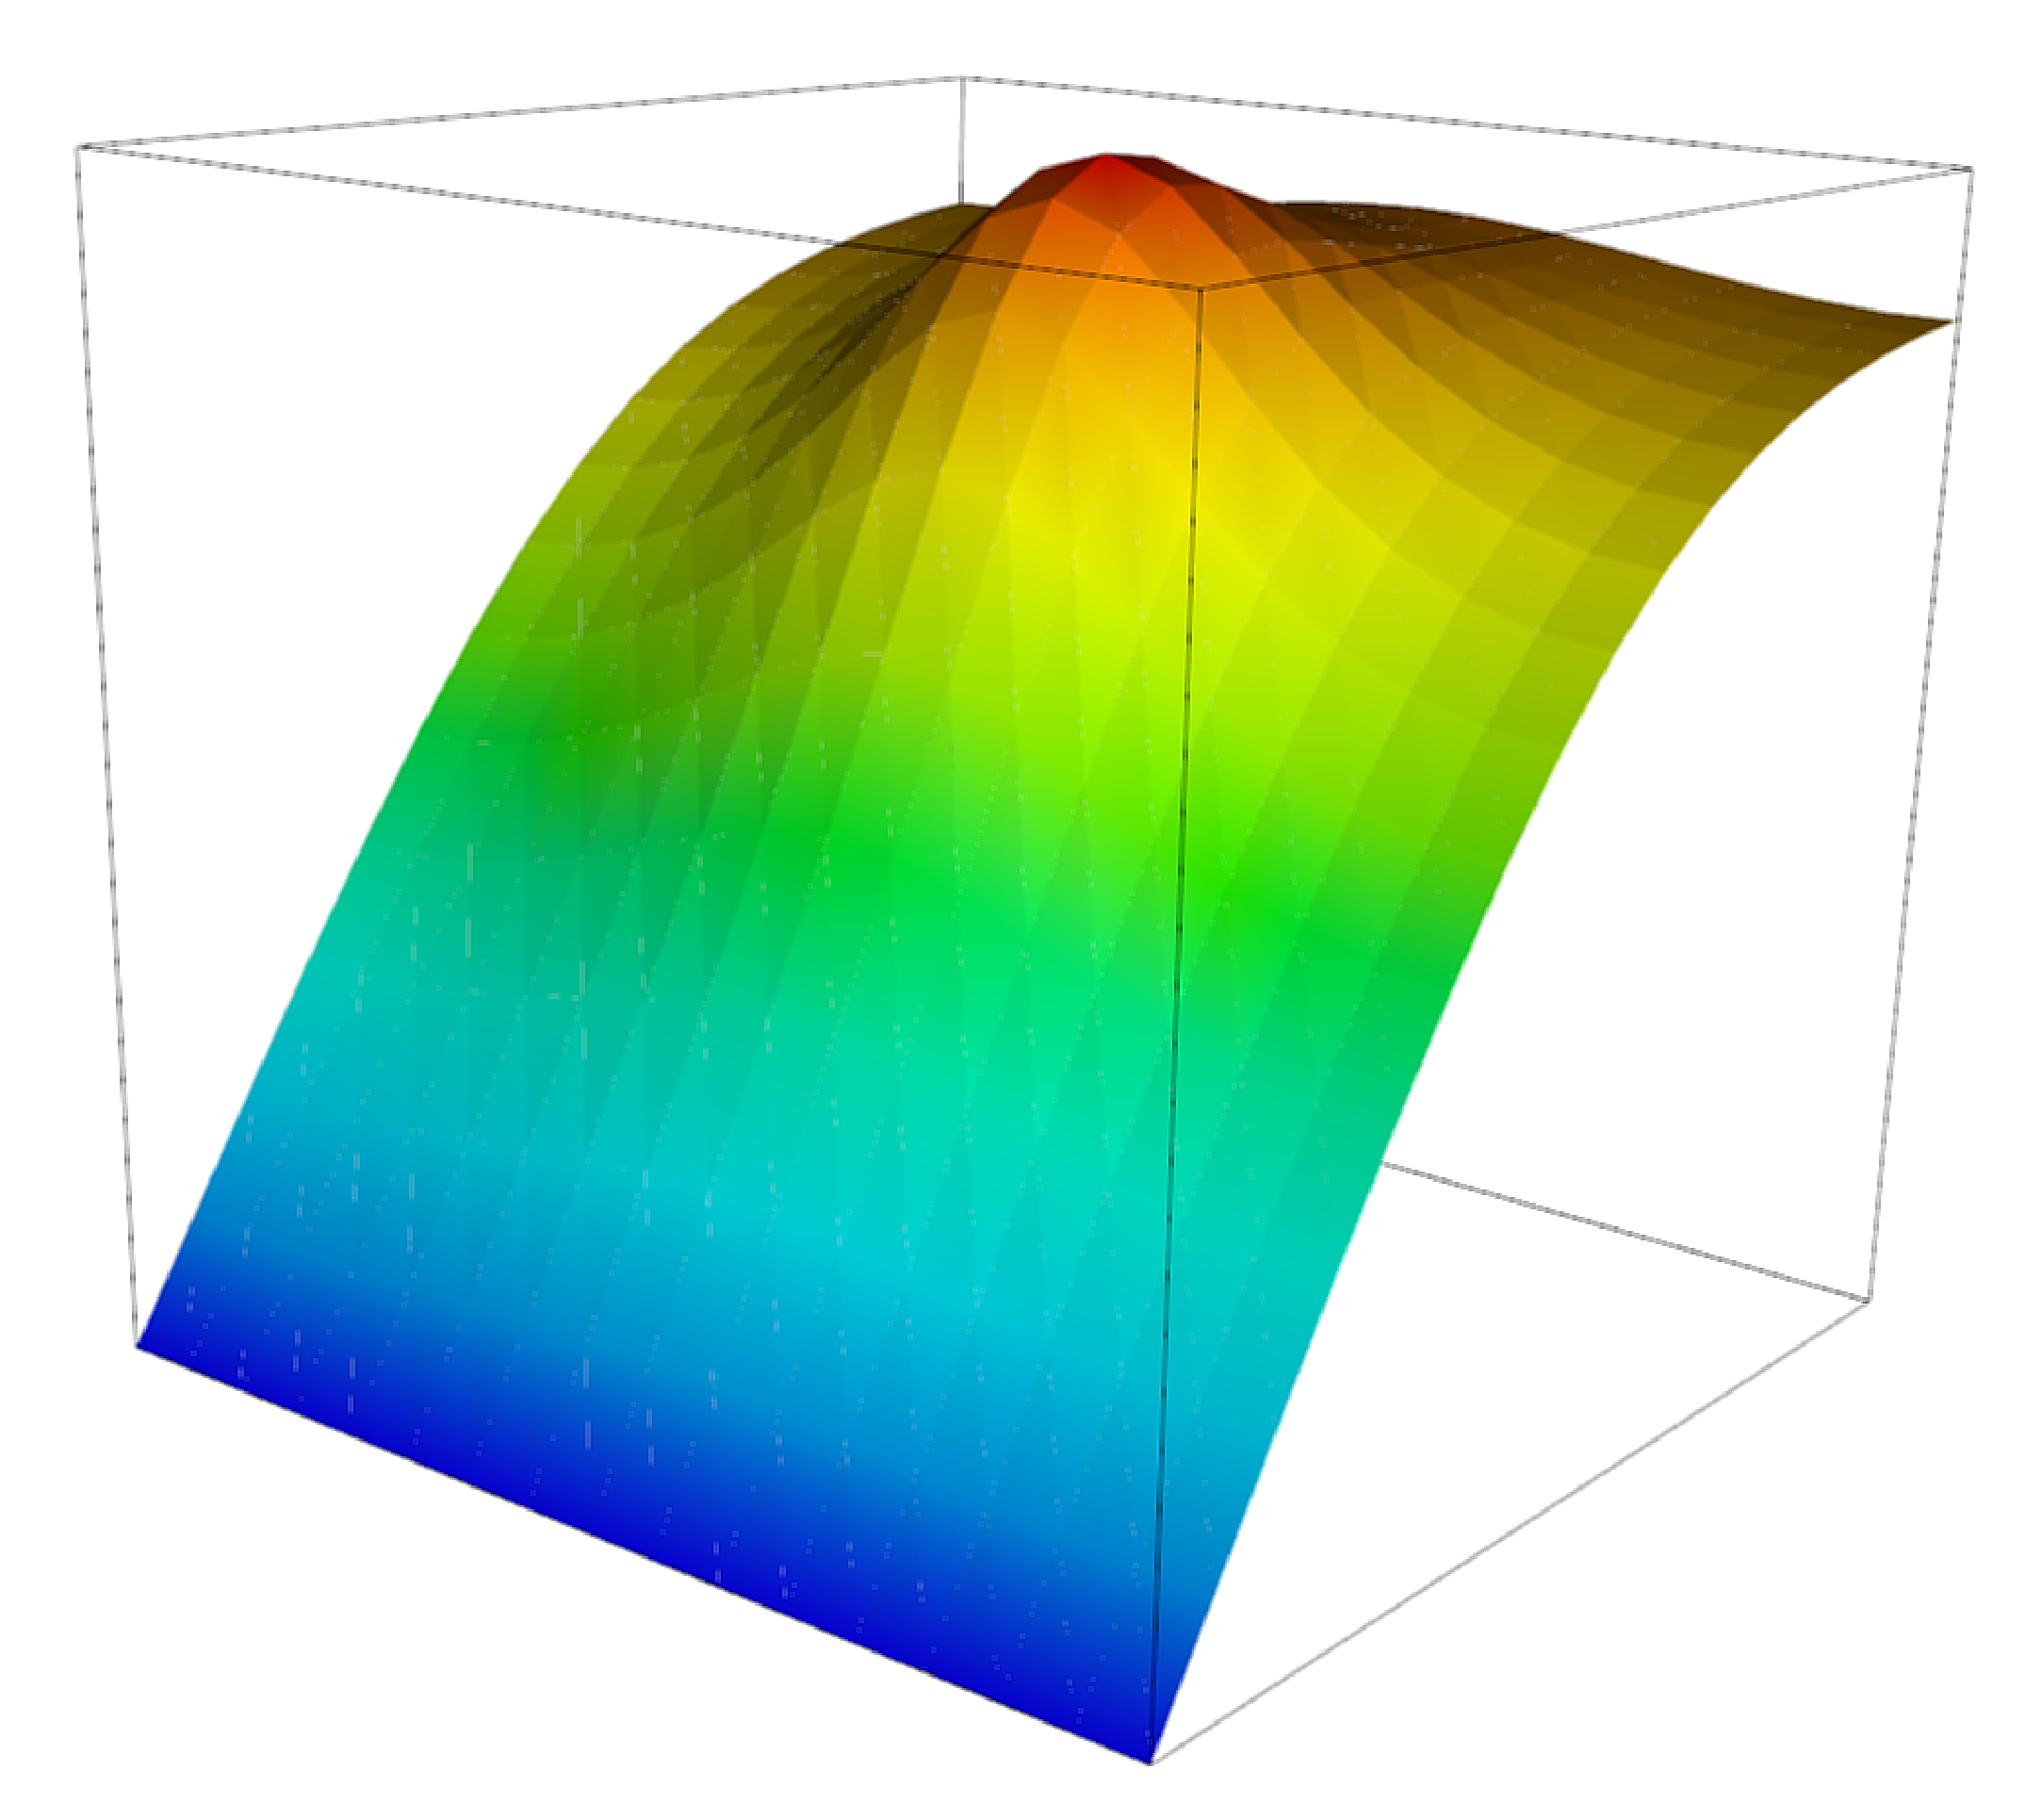
\includegraphics[width=12cm]{eps/poisson.eps}
    \caption{The solution of Poisson's equation (\ref{eq:poisson,quickstart})
      visualized in Octave.}
  \end{center}
\end{figure}

\chapter{Linear algebra}

\devnote{Since this chapter was written, the \dolfin{} linear algebra
  interface has undergone some changes that are not documented here.
  As a result, some of the information in this chapter may be
  outdated, incomplete or simply wrong.}

\dolfin{} provides a high-performance linear algebra library,
including matrices and vectors, a set of linear solvers,
preconditioners, and an eigenvalue solver. The core part of the
functionality is provided through wrappers that provide a common
interface to the functionality of the linear algebra libraries
uBLAS~\cite{www:ublas}, PETSc~\cite{www:petsc} and 
Trilinos~\cite{www.trilonos}.

%------------------------------------------------------------------------------
\section{Matrices and vectors}
\index{\texttt{Matrix}}
\index{\texttt{Vector}}

The two basic linear algebra data structures are the classes
\texttt{Matrix} and \texttt{Vector}, representing a sparse $M\times
N$ matrix and a vector of length $N$ respectively.

The following code demonstrates how to create a matrix and a vector:
\begin{code}
Matrix A(M, N);
Vector x(N);
\end{code}
Alternatively, the matrix and the vector may be created by
\begin{code}
Matrix A;
Vector x;

A.init(M, N);
x.init(N);
\end{code}

The following code demonstrates how to access the size and the
elements of a matrix and a vector:
\begin{code}
A(5, 5) = 1.0;
double a = A(4, 3);

x(3) = 2.0;
double b = x(5);

unsigned int M = A.size(0);
unsigned int N = A.size(1);

N = x.size();
\end{code}

In addition, \dolfin{} provides optimized functions for setting the
values of a set of entries in a matrix or vector:
\begin{code}
double block[] = {2, 4, 6};
int rows[] = {0, 1, 2};
int cols[] = {0, 1, 2};
  
A.set(block, rows, cols, 3);
\end{code}
Alternatively, the set of values given by the array \texttt{block} can
be added to the entries given by the arrays \texttt{rows} and
\texttt{cols}:
\begin{code}
double block[] = {2, 4, 6};
int rows[] = {0, 1, 2};
int cols[] = {0, 1, 2};
  
A.add(block, rows, cols, 3);
\end{code}
These functions are particularly useful for efficient assembly of a (sparse)
matrix from a bilinear form.

\subsection{Sparse matrices}
\index{sparse matrix}

The default \dolfin{} class \texttt{Matrix} is a sparse matrix, which
efficiently represents the discretization of a partial differential
equation where most entries in the matrix are zero. Alternatively,
the class \texttt{SparseMatrix} may be used which is identical with
the class \texttt{Matrix}\footnote{The class \texttt{Matrix} is a
\texttt{typedef} for the class \texttt{SparseMatrix}.}.

If \dolfin{} has been compiled with support for PETSc, then the sparse
matrix is represented as a sparse PETSc matrix\footnote{By default, the
sparse matrix is represented as a PETSc \texttt{MATSEQAIJ} matrix, but
other PETSc representations are also available.}. Alternatively, the
class \texttt{PETScMatrix} may be used, together with the corresponding
class \texttt{PETScVector}.

If \dolfin{} has been compiled without support for PETSc, then the
sparse matrix is represented as a uBLAS sparse matrix. Alternatively,
the class \texttt{uBLASSparseMatrix} may be used, together with the
corresponding class \texttt{uBLASVector}.

\subsection{Dense matrices}
\index{dense matrix}

\dolfin{} provides the class \texttt{DenseMatrix} for representation
of dense matrices. A dense matrix representation is often preferable
when computing with matrices of small to moderate size. In particular,
accessing individual elements 
is more efficient with a dense matrix representation.

A \texttt{DenseMatrix} is represented as uBLAS dense matrix and
alternatively the class \texttt{uBLASDenseMatrix} may be used,
together with the corresponding class \texttt{uBLASVector}.

\subsection{The common interface}
\index{\texttt{GenericMatrix}}
\index{\texttt{GenericVector}}

Although \dolfin{} differentiates between sparse and dense data
structures, the two classes \texttt{GenericMatrix} and
\texttt{GenericVector} define a common interface to all matrices and
vectors. Refer to the \emph{DOLFIN programmer's reference} for the
exact specification of these interfaces.

The following points should be noted:
\begin{enumerate}
\item
  If you want a specific backend like PETSc, then use
  \texttt{PETScVector}/\texttt{PETScMatrix}.
\item
  If you don't care about the backend, then use \texttt{Vector}/\texttt{Matrix}.
\item
  If you write a \emph{function} that should be able to accept vectors
  and matrices from any backend as input, then use
  \texttt{GenericVector}/\texttt{GenericMatrix}.
\end{enumerate}

%------------------------------------------------------------------------------
\section{Solving linear systems}
\index{linear systems}

\dolfin{} provides a set of efficient solvers for linear systems of
the form
\begin{equation}
  Ax = b,
\end{equation}
where $A$ is an $N\times N$ matrix and where $x$ and $b$ are vectors
of length $N$. Both iterative (Krylov subspace) solvers and direct
(LU) solvers are provided.

\subsection{Iterative methods}
\index{iterative methods}
\index{\texttt{GMRES}}
\index{GMRES method}
\index{\texttt{KrylovSolver}}
\index{Krylov subspace methods}

A linear system may be solved by the GMRES Krylov method as follows:
\begin{code}
Matrix A;
Vector x, b:

GMRES::solve(A, x, b);
\end{code}
Alternatively, the linear system may be solved by first creating an
object of the class \texttt{KrylovSolver}, which is more efficient for
repeated solution of linear systems and also allows the specification
of both the Krylov method and the preconditioner:
\begin{code}
KrylovSolver solver(gmres, ilu);
solver.solve(A, x, b);
\end{code}

For uBLAS matrices and vectors, the class \texttt{uBLASKrylovSolver}
may be used and for PETSc matrices and vectors, the class
\texttt{PETScKrylovSolver} may be used.

\subsubsection{Krylov methods}
\index{conjugate gradient method}
\index{BiCGStab}

\dolfin{} provides the following set of Krylov methods:

\begin{center}
\begin{tabular}{|l|l|}
\hline
\texttt{cg}              & The conjugate gradient method \\
\hline
\texttt{gmres}           & The GMRES method \\
\hline
\texttt{bicgstab}        & The stabilized biconjugate gradient squared
method \\
\hline
\texttt{default\_method} & Default choice of Krylov method \\
\hline
\end{tabular}
\end{center}

\subsubsection{Preconditioners}
\index{preconditioners}
\index{ILU}
\index{incomplete LU factorization}
\index{SOR}
\index{successive over-relaxation}
\index{Jacobi}
\index{AMG}
\index{algebraic multigrid}

\dolfin{} provides the following set of preconditioners:

\begin{center}
\begin{tabular}{|l|l|}
\hline
\texttt{none}        & No preconditioning \\
\hline
\texttt{jacobi}      & Simple Jacobi preconditioning \\
\hline
\texttt{sor}         & SOR, successive over-relaxation \\
\hline
\texttt{ilu}         & Incomplete LU factorization \\
\hline
\texttt{icc}         & Incomplete Cholesky factorization \\
\hline
\texttt{amg}         & Algebraic multigrid (through Hypre when available) \\
\hline
\texttt{default\_pc} & Default choice of preconditioner \\
\hline
\end{tabular}
\end{center}

\subsubsection{Matrix-free solvers}
\index{matrix-free solvers}
\index{virtual matrix}

The \dolfin{} Krylov solvers may be used without direct access to a
matrix representation. All that is needed is to provide the
size of the linear system, the right-hand side, and a method
implementing the multiplication of the matrix with any given vector.

Such a ``virtual matrix'' may be defined by implementing the
interface defined by either the class \texttt{uBLASKrylovMatrix} of
\texttt{PETScKrylovMatrix}. The matrix may then be used together with
either the class \texttt{uBLASKrylovSolver} or \texttt{PETScKrylovSolver}.

\subsection{Direct methods}
\index{\texttt{LU}}
\index{\texttt{LUSolver}}
\index{direct methods}
\index{LU factorization}

A linear system may be solved by a direct LU factorization as follows:
\begin{code}
Matrix A;
Vector x, b;
  
LU::solve(A, x, b);
\end{code}
Alternatively, the linear system may be solved by first creating an
object of the class \texttt{LUSolver}, which may be more efficient for
repeated solution of linear systems:
\begin{code}
LUSolver solver;
solver.solve(A, x, b);
\end{code}

For uBLAS matrices and vectors, the class \texttt{uBLASLUSolver} may
be used and for PETSc matrices and vectors, the class
\texttt{PETScLUSolver} may be used.

%------------------------------------------------------------------------------
\section{Eigenvalue problems}
\index{eigenvalue problems}
\index{SLEPc}

\dolfin{} also provides a solver for eigenvalue problems\index{eigenvalue solver}. 
The solver is only available when \dolfin{} has been compiled with support for 
PETSc and SLEPc~\cite{www:slepc}.

For the basic eigenvalue problem
%
\begin{equation}
  Ax = \lambda x,
\end{equation}
%
the following code demonstrates how to compute the first eigenpair:
%
\begin{code} 
SLEPcEigenvalueSolver esolver; 
esolver.solve(A);

double lr, lc;
PETScVector xr, xc;
esolver.getEigenpair(lr, lc, xr, xc, 0);
\end{code} 
%
The double and complex components of the eigenvalue are returned in \texttt{lr}
and \texttt{lc}, respectively, and the double and complex parts of the eigenvector
are returned in \texttt{xr} and \texttt{xc}, respectively.

For the generalized eigenvalue problem
\begin{equation}
 A x = \lambda B x,
\end{equation}
the following code demonstrates how to compute the third eigenpair:
\begin{code} 
PETScEigenvalueSolver esolver; 
esolver.solve(A, B);

double lr, lc;
PETScVector xr, xc;
esolver.getEigenpair(lr, lc, xr, xc, 2);
\end{code} 
%------------------------------------------------------------------------------
\section{Linear algebra backends}
\index{linear algebra backends}

\subsection{uBLAS}
\index{uBLAS}

uBLAS is a C++ template library that provides BLAS level 1, 2 and 3
functionality (and more) for dense, packed and sparse matrices.
The design and implementation unify mathematical notation via operator
overloading and efficient code generation via expression templates.

\dolfin{} wrappers for uBLAS linear algebra is provided through the
classes \texttt{uBLASSparseMatrix}, \texttt{uBLASDenseMatrix} and
\texttt{uBLASVector}. These classes are implemented by subclassing the
corresponding uBLAS classes, which means that all standard
\texttt{uBLAS} operations are supported for these classes. For
advanced usage not covered by the common \dolfin{} interface specified
by the classes \texttt{GenericMatrix} and \texttt{GenericVector},
refer directly to the documentation of \texttt{uBLAS}.
%------------------------------------------------------------------------------
\subsection{PETSc}
\index{PETSc}
%
PETSc is a suite of data structures and routines for the scalable
(parallel) solution of scientific applications modeled by partial
differential equations. It employs the MPI standard for all 
message-passing communication.

\dolfin{} wrappers for PETSc linear algebra is provided through the
classes \texttt{PETScMatrix} and \texttt{PETScVector}. Direct access
to the PETSc data structures is available through the member functions
\texttt{mat()} and \texttt{vec()}, which return the PETSc \texttt{Mat}
and \texttt{Vec} pointers respectively. For advanced usage not covered
by the common \dolfin{} interface specified by the classes
\texttt{GenericMatrix} and \texttt{GenericVector}, refer directly to
the documentation of PETSc.

%------------------------------------------------------------------------------
\subsection{Trilinos}
\index{Trilinos}
%
Trilinos . . . . 
%------------------------------------------------------------------------------
\subsection{Matrix Template Library (MTL4)}
\index{MTL4}
\index{Matrix Template Library}
%
MTL4 . . . . 
%------------------------------------------------------------------------------
\subsection{User provided linear algebra backends}
\index{Trilinos}
%
\devnote{This section will explain how a user-provided linear alegra backend
          can be used with \dolfin{}.}


\chapter{The mesh}

\devnote{The \dolfin{} mesh library has recently been reimplemented
  from scratch and replaces the old mesh library starting at \dolfin{}
  version 0.6.3.  The new mesh is simpler, faster and more general
  than the old mesh library, but adaptive mesh refinement is still
  missing from the old feature set. This will be added in the near
  future.}

\devnote{This chapter is just a quick write-up of the most basic
  functionality of the mesh library and will be expanded.}

\newpage

\section{Basic concepts}

\subsection{Mesh}

A \emph{mesh} consists of \emph{mesh topology} and \emph{mesh geometry}.
These concepts are implemented by the classes \texttt{Mesh},
\texttt{MeshTopology} and \texttt{MeshGeometry}.

\subsection{Mesh entities}

A \emph{mesh entity} is a pair $(d, i)$, where $d$ is the topological
dimension of the mesh entity and $i$ is a unique index of the mesh
entity. Mesh entities are numbered within each topological dimension
from $0$ to $n_d-1$, where $n_d$ is the number of mesh entities of
topological dimension $d$.

For convenience, mesh entities of topological dimension $0$ are
referred to as \emph{vertices}, entities of dimension $1$
\emph{edges}, entities of dimension $2$ \emph{faces}, entities of
\emph{codimension} $1$ \emph{facets} and entities of codimension $0$
\emph{cells}. These concepts are summarized in
Table~\ref{tab:entities}.

\begin{table}[htbp]
  \begin{center}
    \begin{tabular}{|l|c|c|}
      \hline
      Entity & Dimension & Codimension \\
      \hline
      Vertex & $0$       & -- \\
      Edge   & $1$       & -- \\
      Face   & $2$       & -- \\
      & & \\
      Facet  & --      &  $1$ \\
      Cell   & --      &  $0$ \\
      \hline
    \end{tabular}
    \caption{Named mesh entities.}
    \label{tab:entities}
  \end{center}
\end{table}

These concepts are implemented by the classes
\texttt{MeshEntity},
\texttt{Vertex},
\texttt{Edge},
\texttt{Face},
\texttt{Facet},
\texttt{Cell}.

\section{Mesh iterators}

Algorithms operating on a mesh
can often be expressed in terms of
\emph{iterators}. The mesh library provides the general iterator
\texttt{MeshEntityIterator} for iteration over mesh entities, as well
as the specialized mesh iterators
\texttt{VertexIterator},
\texttt{EdgeIterator},
\texttt{FaceIterator},
\texttt{FacetIterator} and
\texttt{CellIterator}.

The following code illustrates how to iterate over all incident
(connected) vertices of all vertices of all cells of a given mesh:
\begin{code}
  for (CellIterator c(mesh); !c.end(); ++c)
    for (VertexIterator v0(c); !v0.end(); ++v0)
      for (VertexIterator v1(v0); !v1.end(); ++v1)
        cout << *v1 << endl;
\end{code}
This may alternatively be implemented using the general iterator
\texttt{MeshEntityIterator} as follows:
\begin{code}
  unsigned int dim = mesh.topology().dim();
  for (MeshEntityIterator c(mesh, dim); !c.end(); ++c)
    for (MeshEntityIterator v0(c, 0); !v0.end(); ++v0)
      for (MeshEntityIterator v1(v0, 0); !v1.end(); ++v1)
        cout << *v1 << endl;
\end{code}

\section{Mesh functions}

A \texttt{MeshFunction} represents a discrete function that takes a
value on each mesh entity of a given topological dimension.
A \texttt{MeshFunction} may for example be used to store a global
numbering scheme for the entities of a (parallel) mesh, marking
sub domains or boolean markers for mesh refinement.

\section{Mesh refinement}

A mesh may be refined uniformly as follows:
\begin{code}
  mesh.refine();
\end{code}
\dolfin{} does currently not support adaptive mesh refinement, but
this will be supported in future versions.

\section{Working with meshes}

\subsection{Reading a mesh from file}

A mesh may be loaded from a file, either by specifying the file name
to the constructor of the class \texttt{Mesh}:
\begin{code}
  Mesh mesh(''mesh.xml'');
\end{code}
or by creating a \texttt{File} object and streaming to a
\texttt{Mesh}:
\begin{code}
  File file(''mesh.xml'');
  Mesh mesh;
  file >> mesh;
\end{code}
A mesh may be stored to file as follows:
\begin{code}
  File file(''mesh.xml'');
  Mesh mesh;
  file << mesh;
\end{code}

The \dolfin{} mesh XML format has changed in \dolfin{} version
0.6.3. Meshes in the old XML format may be converted to the new XML
format using the script \texttt{dolfin-convert} included in the
distribution of \dolfin{}. For instructions, type
\texttt{dolfin-convert --help}.

\subsection{Extracting a boundary mesh}

For any given mesh, a mesh of the boundary of the mesh (if any) may be
created as follows:
\begin{code}
  BoundaryMesh boundary(mesh);
\end{code}
A \texttt{BoundaryMesh} is itself a \texttt{Mesh} of the same
geometrical dimension and has the topological dimension of the mesh
minus one.

The computation of a boundary mesh may also provide mappings from the
vertices of the boundary mesh to the corresponding vertices in the
original mesh, and from the cells of the boundary mesh to the
corresponding facets of the original mesh:
\begin{code}
  MeshFunction<unsigned int> vertex_map,
  MeshFunction<unsigned int> cell_map;
  BoundaryMesh boundary(mesh, vertex_map, cell_map);
\end{code}

\subsection{Built-in meshes}

\dolfin{} provides functionality for creating simple meshes, such as
the mesh of the unit square and the unit cube. The following code
demonstrates how to create a $16\times 16$ triangular mesh of the unit square
(consisting of $2\times 16\times 16 = 512$ triangles) and a
$16\times 16\times 16$ tetrahedral mesh of the unit cube (consisting
of $6\times 16\times 16\times 16 = 24576$ tetrahedra):
\begin{code}
  UnitSquare mesh2D(16, 16);
  UnitCube mesh3D(16, 16, 16);
\end{code}

\devnote{We could easily add other built-in meshes, like the unit
  interval, the unit disc, the unit sphere, rectangles, blocks etc.
  Any contributions are welcome.}

\subsection{Creating meshes}

Simplicial meshes (meshes consisting of intervals, triangles or
tetrahedra) may be constructed explicitly by specifying the
cells and vertices of the mesh. A specialized interface for creating
simplicial meshes is provided by the class \texttt{MeshEditor}.
The following code demonstrates how to create a very simple mesh
consisting of two triangles covering the unit square:
\begin{code}
  Mesh mesh;
  MeshEditor editor(mesh, CellType::triangle, 2, 2);
  editor.initVertices(4);
  editor.initCells(2);
  editor.addVertex(0, 0.0, 0.0);
  editor.addVertex(1, 1.0, 0.0);
  editor.addVertex(2, 1.0, 1.0);
  editor.addVertex(3, 0.0, 1.0);
  editor.addCell(0, 0, 1, 2);
  editor.addCell(1, 0, 2, 3);
  editor.close();
\end{code}
Note that the \dolfin{} mesh library is not specialized to simplicial
meshes, but supports general collections of mesh entities. However,
tools like mesh refinement and mesh editors are currently only
available for simplicial meshes.

\chapter{Functions}
\index{functions}
\index{Function}

\devnote{Since this chapter was written, the \texttt{Function} class has
  seen a number of improvements which are not covered here. Chapter needs
  to be updated.}

The central concept of a function on a domain $\Omega \subset \R^d$ is
modeled by the class \texttt{Function}, which is used in \dolfin{} to
represent coefficients or solutions of partial differential equations.

%------------------------------------------------------------------------------
\section{Basic properties}

The following basic properties hold for all \texttt{Function}s:
\begin{itemize}
\item
  A \texttt{Function} can be scalar or vector-valued;
\item
  A \texttt{Function} can be evaluated at each \texttt{Vertex} of a \texttt{Mesh};
\item
  A \texttt{Function} can be restricted to each local \texttt{Cell} of a \texttt{Mesh};
\item
  The underlying representation of a \texttt{Function} may vary.
\end{itemize}

Depending on the actual underlying representation of a \texttt{Function}, it
may also be possible to evaluate a \texttt{Function} at any given \texttt{Point}.

\subsection{Representation}

Currently supported representations of \texttt{Function}s include
\emph{discrete} \texttt{Function}s and \emph{user-defined}
\texttt{Function}s. These are discussed in detail below.

\subsection{Evaluation}

All \texttt{Function}s can be evaluated at the \texttt{Vertices} of a
\texttt{Mesh}. The following example illustrates how to evaluate a
scalar \texttt{Function} at each \texttt{Vertex} of a given
\texttt{Mesh}:
\begin{code}
  Function u;
  Mesh mesh;

  for (VertexIterator vertex(mesh); !vertex.end(); ++vertex)
    cout << ``Value at vertex `` << *vertex << ``: ``
         << u(*vertex) << endl;
\end{code}

If the \texttt{Function} is vector-valued, an additional argument is
needed to specify the component.  The following example illustrates
how to evaluate all components of a vector-valued \texttt{Function}
at all each \texttt{Vertex} of a given \texttt{Mesh}:
\begin{code}
  Function u;
  Mesh mesh;

  for (VertexIterator vertex(mesh); !vertex.end(); ++vertex)
    for (unsigned int i = 0; i < u.vectordim(); i++)
      cout << ``Value of component `` << i << `` at vertex ``
           << *vertex << ``: `` << u(*vertex, i) << endl;
\end{code}

If allowed by the underlying representation, a \texttt{Function}
\texttt{u} may also be evaluated directly at any given \texttt{Point}:
\begin{code}
  Point p(0.5, 0.5, 0.5);
  cout << ``Value at p = `` << p << ``: `` << u(p) << endl;
\end{code}
As in the case of evaluation at a \texttt{Vertex}, the component index
may be given as an additional argument for a vector-valued \texttt{Function}.

\subsection{Assignment}

One \texttt{Function} may be assigned to another \texttt{Function}:
\begin{code}
  Function v;
  Function u = v;
\end{code}
Assignment creates a new \texttt{Function} sharing the same data.  In
particular, this means that modifying the data of one of the two
\texttt{Function}s will also affect the other \texttt{Function}.

\subsection{Components and sub functions}

If a \texttt{Function} is vector-valued, a new \texttt{Function} may be
created to represent any given component of the original \texttt{Function},
as illustrated by the following example:
\begin{code}
  Function u;         // Function with three components
  Function u0 = u[0]; // first component
  Function u1 = u[1]; // second component
  Function u2 = u[2]; // third component
\end{code}

If a \texttt{Function} represents a \emph{mixed} function (one defined in terms
of a mixed \texttt{FiniteElement}, see below), then indexing has the effect of
picking out sub functions. With \texttt{w} a \texttt{Function} representing the
solution $w = (u, p)$ of a Stokes or Navier-Stokes system (with $u$ the vector-valued
velocity and $p$ the scalar pressure), the following example illustrates how to
pick sub functions and components of \texttt{w}:
\begin{code}
  Function w; // mixed Function (u, p)
  u = w[0];   // first sub function (velocity)
  p = w[1];   // second sub function (pressure)
  u0 = u[0];  // first component of the velocity
  u1 = u[1];  // second component of the velocity
  u2 = u[2];  // third component of the velocity
\end{code}

Note that picking a component or sub function creates a new
\texttt{Function} that shares data with the original \texttt{Function}.

\subsection{Output}
\index{ParaView}
\index{MayaVi}

A \texttt{Function} can be written to a file in various file formats.
To write a \texttt{Function}~\texttt{u} to file in VTK~format,
suitable for viewing in ParaView or MayaVi, create a file with
extension \texttt{.pvd}:
\begin{code}
  File file(``solution.pvd'');
  file << u;
\end{code}

For further details on available file formats, see
Chapter~\ref{chapter:io}.

%------------------------------------------------------------------------------
\section{Discrete functions}

A \emph{discrete} \texttt{Function} is defined in terms of a \texttt{Vector} of nodal
values (degrees of freedom), a \texttt{Mesh} and
a \texttt{FiniteElement} specifying the distribution of the nodal values
on the \texttt{Mesh}. In particular, a discrete \texttt{Function}
is given by a linear combinations of basis functions:
\begin{equation}
  v = \sum_{i=1}^{N} v_i \phi_{i},
\end{equation}
where $\{\phi_i\}_{i=1}^N$ is the global basis of the finite element
space defined by the \texttt{Mesh} and the \texttt{FiniteElement}, and
the nodal values $\{v_i\}_{i=1}^N$ are given by the values of a
\texttt{Vector}.

Note that a \emph{discrete} \texttt{Function} may not be evaluated at
arbitrary points (only at each \texttt{Vertex} of a \texttt{Mesh}).

\subsection{Creating a discrete function}

A discrete \texttt{Function} can be initialized in several ways.
In the simplest case, only a \texttt{Vector} \texttt{x} of nodal
values needs to be specified:
\begin{code}
  Vector x;

  Function u(x);
\end{code}
If possible, \dolfin{} will then automatically try to determine the
\texttt{Mesh} and the \texttt{FiniteElement}.

In some cases, it is necessary to also supply a \texttt{Mesh}
when initializing a discrete \texttt{Function}:
\begin{code}
  Vector x;
  Mesh mesh;

  Function u(x, mesh);
\end{code}
If possible, \dolfin{} will then automatically try to determine the
\texttt{FiniteElement}.

In general however, a discrete \texttt{Function} must be initialized
from a given \texttt{Vector}, a \texttt{Mesh}
and a \texttt{FiniteElement}:
\begin{code}
  Vector x;
  Mesh mesh;
  FiniteElement element;

  Function u(x, mesh, element);
\end{code}

\subsection{Accessing discrete function data}

It is possible to access the data of a discrete \texttt{Function},
including the associated \texttt{Vector}, \texttt{Mesh}
and \texttt{FiniteElement}:
\begin{code}
  Vector& x              = u.vector();
  Mesh& mesh             = u.mesh();
  FiniteElement& element = u.element();
\end{code}

\subsection{Attaching discrete function data}

After a discrete \texttt{Function} has been initialized, it is
possible to associate or reassociate data with the \texttt{Function}:
\begin{code}
  Vector x;
  Mesh mesh;
  FiniteElement element;

  Function u(x);
  u.attach(mesh);
  u.attach(element);
\end{code}

Usually, the \texttt{FiniteElement} is given by the
\texttt{BilinearForm} defining the problem. Considering the Poisson
example in Chapter~\ref{chap:quickstart}, a \texttt{Function}
\texttt{u} representing the solution can be initialized as follows:
\begin{code}
  Vector x;
  Mesh mesh;
  Function u(x, mesh);

  Poisson::BilinearForm a;

  FiniteElement& element = a.trial();
  u.attach(element); 
\end{code}
In this example, the \texttt{Function}~\texttt{u} represents a
function in the trial space for the \texttt{BilinearForm}~\texttt{a}.

%------------------------------------------------------------------------------
\section{User-defined functions}
\index{user-defined functions}

In the simplest case, a user-defined \texttt{Function} is just an
expression in terms of the coordinates and is typically used for
defining source terms and initial conditions. For example, a source
term could be given by
\begin{equation} \label{eq:functionexample}
  f = f(x, y, z) = xy \sin(z / \pi).
\end{equation}

There are two ways to create a user-defined \texttt{Function}; either
by creating a sub class of \texttt{Function} or by creating a
\texttt{Function} from a given function pointer.

\subsection{Creating a sub class}

A user-defined \texttt{Function} may be defined by creating a sub
class of \texttt{Function} and overloading the \texttt{eval()}
function.  The following example illustrates how to create a
\texttt{Function} representing the function in
(\ref{eq:functionexample}):
\begin{code}
  class Source : public Function
  \{
    real eval(const Point& p, unsigned int i)
    \{
      return x*y*sin(z / DOLFIN_PI);
    \}
  \};

  Source f;
\end{code}

To create a vector-valued \texttt{Function}, the vector dimension must
be supplied to the constructor of \texttt{Function}:
\begin{code}
  class Source : public Function
  \{
  public:

    Source() : Function(3) \{\}

    real eval(const Point& p, unsigned int i)
    \{
      if ( i == 0 )
        return 0.0;
      else if ( i == 1 )
        return x*y*sin(z / DOLFIN_PI);
      else
        return x + y;
    \}
  \};

  Source f;
\end{code}

\subsection{Specifying a function-pointer}

A user-defined \texttt{Function} may alternatively be defined by
specifying a function pointer. The following example illustrates
an alternative way of creating a \texttt{Function} representing the
function in (\ref{eq:functionexample}):
\begin{code}
  real source(const Point& p, unsigned int i)
  \{
    return x*y*sin(z / DOLFIN_PI);
  \}

  Function f(source);
\end{code}

As before, for vector-valued \texttt{Function}s, the vector dimension
must be supplied to the constructor of \texttt{Function}:
\begin{code}
  real source(const Point& p, unsigned int i)
  \{
    if ( i == 0 )
      return 0.0;
    else if ( i == 1 )
      return x*y*sin(z / DOLFIN_PI);
    else
      return x + y;
  \}
  
  Function f(source, 3);
\end{code}

\subsection{Cell-dependent functions}

In some cases, it may be convenient to define a \texttt{Function} in
terms of properties of the current \texttt{Cell}. One such example is
a \texttt{Function} that at any given point takes the value of the
mesh size at that point.

The following example illustrates how to create such as
\texttt{Function} by overloading the \texttt{eval()} function:
\begin{code}
  class MeshSize : public Function
  \{
    real eval(const Point& p, unsigned int i)
    \{
      return cell().diameter();
    \}
  \}

  MeshSize h;
\end{code}

Note that the current \texttt{Cell} is only available during assembly
and has no meaning otherwise. It is thus not possible to write the
\texttt{Function}~\texttt{h} to file, since the current \texttt{Cell}
is not available when evaluating a \texttt{Function} at any given
\texttt{Vertex}. Furthermore, note that the current \texttt{Cell} is
not available when creating a \texttt{Function} from a function pointer.

%------------------------------------------------------------------------------
\section{Time-dependent functions}

\devnote{Write about time-dependent and pseudo time-dependent functions.}

\chapter{Ordinary differential equations}

\devnote{This chapter needs to be written. In the meantime, checkout the demos
  in \texttt{src/demo/ode/} and the base class \texttt{ODE}.}


% FIXME: Mono-adaptive, multi-adaptive, ODE base class, simple example,
% FIXME: error control, adaptivity, complex ODE, implicit, homotopies

\chapter{Partial differential equations}
\label{sec:pde}
\index{partial differential equations}

\section{Boundary value problems}

As a prototype of a boundary value problem in $\Bbb{R}^d$ we consider the 
scalar Poisson equation with homogeneous Dirichlet boundary conditions 
\begin{eqnarray}
-\Delta u(x)&=&f(x) \quad x\in \Omega \subset \Bbb{R}^d \label{pde:poisson:strong} \\
u(x)&=&0 \quad x\in \partial \Omega. \nonumber  
\end{eqnarray}

\section{Variational formulation}

A variational formulation of (\ref{pde:poisson:strong}) take the form: 
find $u\in V$ such that  
\begin{equation}\label{pde:poisson:weak}
a(u,v)=L(v) \quad \forall v\in V, 
\end{equation}
where $a(\cdot,\cdot):V\times V\rightarrow \Bbb{R}$ is a bilinear form 
on $V$ defined by 
\begin{equation}
a(u,v)=\int_{\Omega} \nabla u \cdot \nabla v ~dx 
=\int_{\Omega} \frac{\partial u}{\partial x_i} \frac{\partial v}{\partial x_i} ~ dx,  
\end{equation}
where we employ tensor notation so that the double index $i$ means summation from $i=1,...,d$, 
and $L(\cdot):V\rightarrow \Bbb{R}$ is a linear form on $V$ defined by 
\begin{equation}
L(v)=\int_{\Omega} f v ~dx.  
\end{equation}
$V=H^1_0(\Omega)$ is the standard Sobolev space of square integrable 
functions with also their first derivatives square integrable (in the Lebesgue sense), 
with the functions being zero on the boundary (in the sense of traces).   

The Finite Element Method FEM for (\ref{pde:poisson:weak}) is now: 
find $U\in V_h$ such that  
\begin{equation}\label{pde:poisson:fem}
a(U,v)=L(v) \quad \forall v\in V_h, 
\end{equation}
where $V_h\subset V$ is a finite dimensional subspace of dimension $N$. 
The finite element space $V_h$ is characterized by the set of basis 
functions $\{\varphi_i\}_{i=1}^N$, and thus the FEM method 
(\ref{pde:poisson:fem}) is specified by the variational form and 
the basis functions of $V_h$. 

\section{Compiling the variational form with FFC}

In \dolfin{} a PDE is defined in variational form using tensor notation 
in a \texttt{.form} file, which is compiled using FFC. 

In FFC, (\ref{pde:poisson:fem}) is defined by:  
\begin{code}
element = FiniteElement("Lagrange", "tetrahedron", 1)

v = BasisFunction(element)
u = BasisFunction(element)
f = Function(element)

a = v.dx(i)*u.dx(i)*dx
L = v*f*dx
\end{code}

Compiling the file with 
\begin{code}
# ffc Poisson.form
\end{code}
generate a file \texttt{Poisson.h} containing the classes 
\texttt{BilinearForm} and \texttt{LinearForm}, and 
classes for the finite element used in the forms. 

\section{Assemble matrices and vectors}

The class \texttt{FEM} automates the assembly algorithm, constructing a linear 
system of equations from a given partial differential equation, 
given in the form of a variational problem (\ref{pde:poisson:weak}), 
with a bilinear form $a(\cdot,\cdot)$ and a linear form $L(\cdot)$. 

The classes \texttt{BilinearForm} and \texttt{LinearForm} are automatically 
generated by FFC, and to assemble the corresponding matrix and vector for 
the Poisson problem with source term $f$, we write:  
\begin{code}
Poisson::BilinearForm a;
Poisson::LinearForm L(f);

Mesh mesh; 
Mat A;
Vec b;

FEM::assemble(a,L,A,b,mesh);
\end{code}

In the \texttt{assemble} function the element matrices and vectors are 
computed by calling the function \texttt{eval} in the classes 
\texttt{Bilinearform} and \texttt{Linearform}. 
The \texttt{eval} function at a certain element in the assebly algorithm 
takes as argument an \texttt{AffineMap} object, 
describing the mapping from the reference element to the actual element, 
by computing the jacobian $J$ of the mapping (also $J^{-1}$ and $det(J)$ 
are computed).  

\section{Boundary conditions}

\section{Finite elements}

Finite Element by Ciarlet, FIAT, FFC  

\section{Computation of Element matrices and vectors} 

divide element matrix into geometry tensor and integration 
over reference element FErari

precomputation of integrals, quadrature, tensorrepresentation factored out, FFC 

\section{Initial value problems}

semidiscretization, space-time FEM, 

% Insert note that constants are passed into forms as references

\chapter{Nonlinear solver}
\index{nonlinear solver}

\dolfin{} provides tools for solving nonlinear equations of the form
\begin{equation}
  F(u) = 0, 
\end{equation}
where $F: \mathbb{R}^{n} \rightarrow \mathbb{R}^{n}$. 
To use the nonlinear solver, a nonlinear function must be defined. 
The nonlinear solver is then initialised with this function and a 
solution computed.

\section{Nonlinear functions}
\index{NonlinearFunction}

To solve a nonlinear problem, the user must defined a class which 
represents the nonlinear function $F(u)$. The class 
should be derived from the \dolfin{}  class \texttt{NonlinearFunction}. It
contains the necessary functions to form the function $F(u)$ and the 
Jacobian matrix  $J = \partial F / \partial u$. The precise form of the user 
defined class will depend on the problem being solved.
The structure of a user defined class \texttt{MyNonlinearFunction} is shown below.
%
\begin{code}
class MyNonlinearFunction : public NonlinearFunction
{
public: 
  
 // Constructor 
 MyNonlinearFunction() : NonlinearFunction() {}
  
 // Compute F(u) and J 
 void form(GenericMatrix& A, GenericVector& b, 
           const GenericVector& u)
 {
   // Insert F(u) into the vector b and J into the matrix A 
 }

private:
 // Functions and pointers to objects with which F(u) is defined
};
\end{code}
%
The above class computes the function $F(u)$ and its Jacobian $J$
concurrently. In the future, it will be possible to compute 
$F(u)$ and $J$ either concurrently or separately.

\section{Newton solver}
\index{Newton's method}
\index{NewtonSolver}
%
\dolfin{} provides tools to solve nonlinear systems using Newton's method
and variants of it. The following code solves a nonlinear problem, defined by 
\texttt{MyNonlinearFunction} using Newton's method.
%
\begin{code}
Vector u;
MyNonlinearFunction F;
NewtonSolver newton_solver;

nonlinear_solver.solve(F, x);
\end{code}
%

The maximum number of iterations before the Newton 
procedure is exited can be set through the \dolfin{} parameter
system, along with the relative and absolute 
tolerances the residual. This is illustrated below.
%
\begin{code}
NewtonSolver nonlinear_solver;
nonlinear_solver.set("Newton maximum iterations", 50);
nonlinear_solver.set("Newton relative tolerance", 1e-10);
nonlinear_solver.set("Newton absolute tolerance", 1e-10);
\end{code}

The Newton procedure is considered to have converged when
the residual $r_{n}$ at iteration $n$ is less than the 
absolute tolerance or the relative residual
$r_{n}/r_{0}$ is less than the relative tolerance.
By default, the residual at iteration $n$ is given
by
%
\begin{equation}
  r_{n} = \| F(u_{n}) \|.
\end{equation} 
%
Computation of the residual in this way can be set by
%
\begin{code}
NewtonSolver newton_solver;
newton_solver.set("Newton convergence criterion", "residual");
\end{code}

For some problems, it is more appropriate to consider changes in
the solution~$u$ in testing for convergence. At iteration $n$,
the solution is updated via
%
\begin{equation}
  u_{n} = u_{n-1} + du_{n} 
\end{equation}
%
where $du_{n}$ is the increment. When using an incremental
criterion for convergence, the `residual' is defined as
%
\begin{equation}
  r_{n} = \| du_{n} \|.
\end{equation} 
%
Computation of the incremental residual can be set by
%
\begin{code}
NewtonSolver newton_solver;
newton_solver.set("Newton convergence criterion", "incremental");
\end{code}
%


\subsection{Linear solver}
The solution to the nonlinear problems is returned in the vector~\texttt{x}.
By default, the \texttt{NewtonSolver} used a direct solver to solve systems
of linear equations. It is possible to set the type linear solver to be used 
when creating a \texttt{NewtonSolver}. For example, 
%
\begin{code}
NewtonSolver newton_solver(gmres);
\end{code}
%
creates a solver which will use GMRES to solve linear systems. For iterative
solvers, the preconditioner can also be selected,
\begin{code}
NewtonSolver newton_solver(gmres, ilu);
\end{code}
%
The above Newton solver will use GMRES in combination with incomplete LU 
factorisation.

\subsection{Application of Dirichlet boundary conditions}
%
The application of Dirichlet boundary conditions to finite element
problems in the context of a Newton solver requires particular 
attention. The `residual' $F(u)$ at nodes where Dirichlet boundary
conditions are applied is the equal to difference between the 
imposed boundary condition value and the current solution~$u$.
The function 
\begin{code}
void FEM::applyResidualBC(GenericVector& b, 
           const GenericVector& x, Mesh& mesh,
           FiniteElement& element, BoundaryCondition& bc)
\end{code}
applies Dirichlet boundary conditions correctly. For a nonlinear
finite element problem, the below code assembles the function $F(u)$
and its Jacobian, and applied Dirichlet boundary conditions in the
appropriate manner.
%
\begin{code}
class MyNonlinearFunction : public NonlinearFunction
{
public: 
  
  // Constructor 
  MyNonlinearFunction(. . . ) : NonlinearFunction(. . . ) {}
  
  // Compute F(u) and J 
  void form(GenericMatrix& A, GenericVector& b, 
            const GenericVector& u)
  {
    // Insert F(u) into the vector b and J into the matrix A 
    FEM::assemble(*a, *L, A, b, *_mesh);
    FEM::applyBC(A, *_mesh, a->test(), *_bc);
    FEM::applyResidualBC(b, x, *_mesh, a->test(), *_bc);
  }

private:
  // Functions and pointers to objects with which F(u) is defined
};
\end{code}

\section{Incremental Newton solver}
%
Newton solvers are commonly used to solve nonlinear equations in a series 
of steps. This can be done by building a simple loop around a Newton solver,
and is shown in the following code.
%
\begin{code}
MyNonlinearProblem F(U);
NewtonSolver nonlinear_solver;

Vector& x = U.vector();

// Solve nonlinear problem in a series of steps
real dt = 1.0; real t  = 0.0; real T  = 3.0;
while( t < T)
{
  t += dt;
  nonlinear_solver.solve(F, x);
}
\end{code}
%
Typically, the boundary conditions and/or source terms will be dependent 
on~\texttt{t}.

\chapter{Input/output}
\label{chapter:io}
\index{input/output}
\index{I/O}
\index{pre-processing}
\index{post-processing}

\dolfin{} relies on external programs for pre- and post-processing,
which means that computational meshes must be imported from file
(pre-processing) and computed solutions must be exported to file and
then imported into another program for visualization
(post-processing). To simplify this process, \dolfin{} provides
support for easy interaction with files and includes output formats
for a number of visualization programs.

%------------------------------------------------------------------------------
\section{Files and objects}
\index{object}
\index{\texttt{File}}

A file in \dolfin{} is represented by the class \texttt{File} and
reading/writing data is done using the standard C++ operators
\texttt{>>} (read) and \texttt{<<} (write).

Thus, if \texttt{file} is a \texttt{File} and \texttt{object} is an
object of some class that can be written to file, then the object can
be written to file as follows:
\begin{code}
  file << object;
\end{code}
Similarly, if \texttt{object} is an object of a class that can be read
from file, then data can be read from file (overwriting any previous
data held by the object) as follows:
\begin{code}
  file >> object;
\end{code}

The format (type) of a file is determined by its filename suffix, if
not otherwise specified. Thus, the following code creates a
\texttt{File} for reading/writing data in \dolfin{} XML format:
\begin{code}
  File file(``data.xml'');
\end{code}
A complete list of file formats and corresponding file name suffixes
is given in Table~\ref{tab:formats}.

Alternatively, the format of a file may be explicitly defined. One may
thus create a file named \texttt{data.xml} for reading/writing data in
GNU~Octave format:
\begin{code}
  File file(``data.xml'', File::octave);
\end{code}

\begin{table}[htbp]
  \begin{center}
    \begin{tabular}{|l|l|l|}
      \hline
      Suffix & Format & Description \\
      \hline
      \hline
      \texttt{.xml}/\texttt{.xml.gz} & \texttt{File::xml} & \dolfin{} XML \\
      \hline
      \texttt{.pvd} & \texttt{File::vtk} & VTK \\
      \hline
      \texttt{.dx} & \texttt{File::opendx} & OpenDX \\
      \hline
      \texttt{.m} & \texttt{File::octave} & GNU Octave \\
      \hline
      (\texttt{.m}) & \texttt{File::matlab} & MATLAB \\
      \hline
      \texttt{.tec} & \texttt{File::tecplot} & Tecplot \\
      \hline
      \texttt{.msh}/\texttt{.res} & \texttt{File::gid} & GiD \\
      \hline
    \end{tabular}
    \caption{File formats and corresponding file name suffixes.}
    \label{tab:formats}
  \end{center}
\end{table}

Although many of the classes in \dolfin{} support file input/output,
it is not supported by all classes and the support varies with the
choice of file format. A summary of supported classes/formats is
given in Table~\ref{tab:classes,formats}.

\devnote{Some of the file formats are partly broken after changing the
  linear algebra backend to PETSc. (Do \texttt{grep FIXME} in \texttt{src/kernel/io/}.)}

\begin{table}[htbp]
  \begin{center}
    \begin{tabular}{|l||c|c|c|c|c|}
      \hline
      Format           & \texttt{Vector} & \texttt{Matrix} & \texttt{Mesh} & \texttt{Function} & \texttt{Sample} \\
      \hline
      \hline
      \texttt{File::xml}     & in/out & in/out & in/out & --- & --- \\
      \hline
      \texttt{File::vtk}     & ---    & ---    & out    & out & --- \\
      \hline
      \texttt{File::opendx}  & ---    & ---    & out    & out & --- \\
      \hline
      \texttt{File::octave}  & out    & out    & out    & out & out \\
      \hline
      \texttt{File::matlab}  & out    & out    & out    & out & out \\
      \hline
      \texttt{File::tecplot} & ---    & ---    & out    & out & ---  \\
      \hline
      \texttt{File::gid}     & ---    & ---    & out    & out & ---\\
      \hline
    \end{tabular}
    \caption{Matrix of supported combinations of classes and file
      formats for input/output in \dolfin{}.}
    \label{tab:classes,formats}
  \end{center}
\end{table}

%------------------------------------------------------------------------------
\section{File formats}
\index{file formats}

In this section, we give some pointers to each of the file formats
supported by \dolfin{}. For detailed information, we refer to the
respective user manual of each format/program.

\devnote{This section needs to be improved and expanded. Any
  contributions are welcome.}

\subsection{\dolfin{} XML}
\index{XML}

\dolfin{} XML is the native format of \dolfin{}. As the name says,
data is stored in XML ASCII format. This has the advantage of being a
robust and human-readable format, and if the files are compressed
there is little overhead in terms of file size compared to a binary
format.

\dolfin{} automatically handles gzipped XML files, as
illustrated by the following example which reads a \texttt{Mesh} from
a compressed \dolfin{} XML file and saves the mesh to an uncompressed
\dolfin{} XML file:
\begin{code}
  Mesh mesh;

  File in(``mesh.xml.gz'');
  in >> mesh;

  File out(``mesh.xml'');
  out << mesh;
\end{code}
The same thing can of course be accomplished by
\begin{code}
  # gunzip -c mesh.xml.gz > mesh.xml
\end{code}
on the command-line.

There is currently no visualization tool that can read \dolfin{} XML
files, so the main purpose of this format is to save and transfer data.

\subsection{VTK}

Data saved in VTK format~\cite{www:VTK} can be visualized using various
packages. The powerful and freely available ParaView~\cite{www:ParaView} 
is recommended. Alternatively, VTK data can be visualized in 
MayaVi~\cite{www:MayaVi}, which is recommended for quality vector PostScript 
output. Time-dependent data is handled automatically in the VTK format.

The below code illustrates how to export a function in VTK format:
\begin{code}
  Function u;

  File out(``data.pvd'');
  out << u;
\end{code}
The sample code produces the file \texttt{data.pvd}, which can be read 
by ParaView. The file \texttt{data.pvd} contains a list of files which 
contain the results computed by \dolfin{}. For the above example, these 
files would be named \texttt{dataXXX.vtu}, where \texttt{XXX} is a counter 
which is incremented each time the function is saved. If the function 
\texttt{u} was to be saved three times, the files
\begin{code}
  data000000.vtu
  data000001.vtu
  data000002.vtu
\end{code}
would be produced. Individual snapshots can be visualized by opening the 
desired file with the extension~\texttt{.vtu} using ParaView.

ParaView can produce on-screen animations. High quality animations 
in various formats can be produced using a combination of ParaView and 
MEncoder~\cite{www:MEncoder}.

\devnote{Add MEncoder example to create animation.}


\subsection{OpenDX}

OpenDX~\cite{www:OpenDX} is a powerful free visualization tool based
on IBM's \emph{Visualization Data Explorer}. To visualize data with
OpenDX, a user needs to build a \emph{visual program} that instructs
OpenDX how to extract and visualize relevant parts of your
data. \dolfin{} provides a ready-made visual program suitable for
visualization of \dolfin{} data in OpenDX. The visual program can be
found in the subdirectory \texttt{src/utils/opendx/} of the \dolfin{}
source tree (file \texttt{dolfin.net} and accompanying configuration
\texttt{dolfin.cfg}).

\subsection{GNU Octave}

GNU~Octave~\cite{www:Octave} is a free clone of MATLAB that can be
used to visualize solutions computed in \dolfin{}, using the commands
\texttt{pdemesh}, \texttt{pdesurf} and \texttt{pdeplot}. These
commands are normally not part of GNU~Octave but are
provided by \dolfin{} in the subdirectory \texttt{src/utils/octave/} of
the \dolfin{} source tree. These commands require the external program
\texttt{ivview} included in the open source distribution of
Open~Inventor~\cite{www:OpenInventor}. (Debian users install the
package \texttt{inventor-clients}.)

To visualize a solution computed with \dolfin{} and exported in
GNU~Octave format, first load the solution into GNU~Octave by just
typing the name of the file without the \texttt{.m} suffix. If the
solution has been saved to the file \texttt{poisson.m}, then just type
\begin{code}
  octave:1> poisson
\end{code}
The solution can now be visualized using the command
\begin{code}
  octave:2> pdesurf(points, cells, u)
\end{code}
or to visualize just the mesh, type
\begin{code}
  octave:3> pdesurf(points, edges, cells)
\end{code}

\subsection{MATLAB}

Since MATLAB~\cite{www:MATLAB} is not free, users are encouraged to
use GNU~Octave whenever possible. That said, data is visualized in
much the same way in MATLAB as in GNU~Octave, using the
MATLAB~commands \texttt{pdemesh}, \texttt{pdesurf} and
\texttt{pdeplot}.

\subsection{Tecplot}

Tecplot~\cite{www:Tecplot} is a proprietary visualization tool.
The Tecplot format is not actively maintained and may be removed in
future versions of \dolfin{} (if there is not sufficient interest to
maintain the format).

\subsection{GiD}

GiD~\cite{www:GiD} is a proprietary visualization tool.
The GiD format is not actively maintained and may be removed in
future versions of \dolfin{} (if there is not sufficient interest to
maintain the format).

%------------------------------------------------------------------------------
\section{Converting between file formats}

\dolfin{} supplies a script for easy conversion between different file
formats.  The script is named \texttt{dolfin-convert} and can be found
in the directory \texttt{src/utils/convert/} of the \dolfin{} source
tree. The only supported file formats are currently the Medit
\texttt{.mesh} format (which can be generated by TetGen) and the
\dolfin{} XML mesh format:
\begin{code}
  # dolfin-convert mesh.mesh mesh.xml
\end{code}

%------------------------------------------------------------------------------
\section{A note on new file formats}

With some effort, \dolfin{} can be expanded with new file formats. Any
contributions are welcome. If you wish to contribute to \dolfin{},
then adding a new file format (or improving upon an existing file
format) is a good place to start. Take a look at one of the current
formats in the subdirectory \texttt{src/kernel/io/} of the \dolfin{}
source tree to get a feeling for how to design the file format, or ask
at \texttt{dolfin-dev@fenics.org} for directions.

Also consider contributing to the \texttt{dolfin-convert} script by
adding a conversion routine for your favorite format. The script is
written in Python and should be easy to extend with new formats.

\chapter{The log system}
\index{log system}

\dolfin{} provides provides a simple interface for uniform handling of
log messages, including warnings and errors. All messages are
collected to a single stream, which allows the destination and
formatting of the output from an entire program, including the
\dolfin{} library, to be controlled by the user.

%------------------------------------------------------------------------------
\section{Generating log messages}
\index{\texttt{message()}}
\index{\texttt{cout}}
\index{\texttt{endl}}

Log messages can be generated using the function
\texttt{message()} available in the \texttt{dolfin} namespace:
\begin{code}
void message(std::string format, ...);
\end{code}
which works similarly to the standard C library function \texttt{printf}.
The following examples illustrate the usage of
\texttt{message()}:
\begin{code}
message("Solving linear system.");
message("Size of vector: \%d.", x.size());
message("R = \%.3e (TOL = \%.3e)", R, TOL);
\end{code}

As an alternative to \texttt{message()}, \dolfin{} provides a C++
style interface to generating log messages. Thus, the above examples
can also be implemented as follows:
\footnotesize
\begin{code}
cout << "Solving linear system." << endl;
cout << "Size of vector: " << x.size() << "." << endl;
cout << "R = " << R << " (TOL = " << TOL << ")" << endl;
\end{code}
\normalsize
Note the use of \texttt{dolfin::cout} and
\texttt{dolfin::endl} from the \texttt{dolfin} namespace,
corresponding to the standard standard \texttt{std::cout} and
\texttt{std::endl} in namespace \texttt{std}. If log messages are
directed to standard output (see below), then \texttt{dolfin::cout}
and \texttt{std::cout} may be mixed freely.

Most classes provided by \dolfin{} can be used together with
\texttt{dolfin::cout} and \texttt{dolfin::endl} to display short
informative messages about objects:
\begin{code}
Matrix A(10, 10);
cout << A << endl;
\end{code}
To display detailed information for an object,  use the member function
\texttt{disp()}:
\begin{code}
Matrix A(10, 10);
A.disp();
\end{code}
Use with caution for large objects. For a \texttt{Matrix}, calling
\texttt{disp()} displays all matrix entries.

%------------------------------------------------------------------------------
\section{Warnings and errors}
\index{warnings}
\index{errors}
\index{\texttt{warning()}}
\index{\texttt{error()}}

Warnings and error messages can be generated using the functions
\begin{code}
warning(std::string format, ...);
error(std::string format, ...);
\end{code}
Once an error is encountered, the program throws an exception.

%------------------------------------------------------------------------------
\section{Debug messages and assertions}
\index{debugging}
\index{assertions}
\index{\texttt{dolfin\_debug()}}
\index{\texttt{dolfin\_assert()}}

The macro \texttt{dolfin\_debug()} works similarly to
\texttt{message()}:
\begin{code}
dolfin_debug(message);
\end{code}
but in addition to displaying the given message, information is printed about
the location of the code that generated the debug message (file,
function name and line number).

Note that in order to pass formatting strings and additional arguments
with debug messages, the variations \texttt{dolfin\_debug1()},
\texttt{dolfin\_debug2()} and so on, depending on the number of
arguments, must be used.

Assertions can often be a helpful programming tool. Use assertions
whenever you assume something about about a variable in your code,
such as assuming that given input to a function is valid. \dolfin{}
provides the macro \texttt{dolfin\_assert()} for creating assertions:
\begin{code}
dolfin_assert(check);
\end{code}
This macro accepts a boolean expression and if the expression
evaluates to false, an error message is displayed, including the
file, function name and line number of the assertion, and a
segmentation fault is raised (to enable easy attachment to a
debugger). The following examples illustrate the use of
\texttt{dolfin\_assert()}:
\begin{code}
dolfin_assert(i >= 0);
dolfin_assert(i < n);
dolfin_assert(cell.type() == Cell::triangle);
dolfin_assert(cell.type() == Cell::tetrahedron);
\end{code}
Note that assertions are only active when compiling
\dolfin{} and your program with \texttt{DEBUG} defined (configure
option \texttt{--enable-debug} or compiler flag \texttt{-DDEBUG}).
Otherwise, the macro \texttt{dolfin\_assert()} expands to nothing,
meaning that liberal use of assertions does not affect performance,
since assertions are only present during development and
debugging.

%------------------------------------------------------------------------------
\section{Task notification}
\index{tasks}
\index{\texttt{dolfin\_begin()}}
\index{\texttt{dolfin\_end()}}

The two functions \texttt{dolfin\_begin()} and \texttt{dolfin\_end()}
available in the \texttt{dolfin} name space can be used to notify the
\dolfin{} log system about the beginning and end of a task:
\begin{code}
void begin();
void end();
\end{code}
Alternatively, a string message (or a formatting string with optional
arguments) can be supplied:
\begin{code}
void begin(std::string format, ...);
void end();
\end{code}

These functions enable the \dolfin{} log system to display messages,
warnings and errors hierarchically, by automatically indenting the
output produced between calls to \texttt{begin()} and
\texttt{end()}. A program may contain an arbitrary number of nested
tasks.

%------------------------------------------------------------------------------
\section{Progress bars}
\index{progress bar}
\index{\texttt{Progress}}

The \dolfin{} log system provides the class \texttt{Progress} for
simple creation of progress sessions. A progress session automatically
displays the progress of a computation using a progress bar.

If the number of steps of a computation is known, a progress session
should  be defined in terms of the number of steps and updated in each
step of the computation as illustrated by the following example:
\begin{code}
Progress p("Assembling", mesh.noCells());  
for (CellIterator c(mesh); !c.end(); ++c)
{
  ...
  p++;
}
\end{code}
It is also possible to specify the step number explicitly by assigning
an integer to the progress session:
\begin{code}
Progress p("Iterating over vector", x.size())
for (uint i = 0; i < x.size(); i++)
{
  ...
  p = i;
}
\end{code}

Alternatively, if the number of steps is unknown, the progress session
needs to be updated with the current percentage of the progress:
\begin{code}
Progress p("Time-stepping");
while ( t < T )
{
  ...
  p = t / T;
}
\end{code}

The progress bar created by the progress session will only be updated
if the progress has changed significantly since the last update (by
default at least $10\%$). The
amount of change needed for an update can be controlled using the
parameter \texttt{"progress step"}:
\begin{code}
dolfin_set("progress step", 0.01);
\end{code}

Note that several progress sessions may be created simultaneously, or
nested within tasks.

%------------------------------------------------------------------------------
\section{Controlling the destination of output}
\index{output destination}

By default, the \dolfin{} log system directs messages to standard
output (the terminal). Messages may also be turned off completely.
To specify the destination, set the value of the parameter "output destination":
\begin{code}
dolfin_set("output destination", "terminal");
dolfin_set("output destination", "silent");
\end{code}

One may also set the debug level for the \dolfin{} log system so that
only messages with a debug level higher than or equal to the current
debug level are printed:
\begin{code}
dolfin_set("debug level", "1");
\end{code}

\chapter{Parameters}
\label{sec:parameters}
\index{parameters}

\devnote{Since this chapter was written, the \dolfin{} parameter system
has been completely redesigned and now supports localization of
parameters to objects or hierarchies of objects. Chapter needs to be updated.}

\dolfin{} keeps a global database of parameters that control the
behavior of the various components of \dolfin{}. Parameters are
controlled using a uniform type-independent interface that allows
retrieving the values of existing parameters, modifying existing
parameters and adding new parameters to the database.

%------------------------------------------------------------------------------
\section{Retrieving the value of a parameter}
\index{\texttt{dolfin\_get()}}

To retrieve the value of a parameter, use the function \texttt{dolfin\_get()}
available in the \texttt{dolfin} namespace:
\begin{code}
Parameter dolfin_get(std::string key);
\end{code}
This function accepts as argument a string \texttt{key} and returns
the value of the parameter matching the given key. An error message is
printed through the log system if there is no parameter with the given
key in the database.

The value of the parameter is automatically cast to the correct type
when assigning the value of \texttt{dolfin\_get()} to a variable, as
illustrated by the following examples:
\begin{code}
double TOL = dolfin_get("tolerance");
int num_samples = dolfin_get("number of samples");
bool solve_dual = dolfin_get("solve dual problem");
std::string filename = dolfin_get("file name");
\end{code}

Note that there is a small cost associated with accessing the value of
a parameter, so if the value of a parameter is to be used multiple
times, then it should be retrieved once and stored in a local variable
as illustrated by the following example:
\begin{code}
int num_samples = dolfin_get("number of samples");
for (int i = 0; i < num_samples; i++)
{
  ...
}
\end{code}

%------------------------------------------------------------------------------
\section{Modifying the value of a parameter}
\index{\texttt{dolfin\_set()}}

To modify the value of a parameter, use the function \texttt{dolfin\_set()}
available in the \texttt{dolfin} namespace:
\begin{code}
void dolfin_set(std::string key, Parameter value);
\end{code}
This function accepts as arguments a string \texttt{key} together with
the corresponding value. The value type should match the type of
parameter that is being modified. An error message is
printed through the log system if there is no parameter with the given
key in the database.

The following examples illustrate
the use of \texttt{dolfin\_set()}:
\begin{code}
dolfin_set("tolerance", 0.01);
dolfin_set("number of samples", 10);
dolfin_set("solve dual problem", true);
dolfin_set("file name", "solution.xml");
\end{code}

Note that changing the values of parameters using
\texttt{dolfin\_set()} does not change the values of already retrieved
parameters; it only changes the values of parameters in the
database. Thus, the value of a parameter must be changed before using
a component that is controlled by the parameter in question.

%------------------------------------------------------------------------------
\section{Adding a new parameter}
\index{\texttt{add()}}

To add a parameter to the database, use the function
\texttt{add()} available in the \texttt{dolfin}
namespace:
\begin{code}
void add(std::string key, Parameter value);
\end{code}
This function accepts two arguments:
a unique key identifying the new parameter and the value of the new
parameter.

The following examples illustrate the use of
\texttt{add()}:
\begin{code}
add("tolerance", 0.01);
add("number of samples", 10);
add("solve dual problem", true);
add("file name", "solution.xml");
\end{code}

%------------------------------------------------------------------------------
\section{Saving parameters to file}
\index{XML}

The following code illustrates how to save the current database of
parameters to a file in \dolfin{} XML format:
\begin{code}
File file("parameters.xml");
file << ParameterSystem::parameters;
\end{code}
When running a simulation in \dolfin{}, saving the parameter database
to a file is an easy way to document the set of parameters used in the
simulation.

%------------------------------------------------------------------------------
\section{Loading parameters from file}
\index{XML}

The following code illustrates how to load a set of parameters into
the current database of parameters from a file in \dolfin{} XML format:
\begin{code}
File file("parameters.xml");
file >> ParameterSystem::parameters;
\end{code}
The following example illustrates how to specify a list of parameters
in the \dolfin{} XML format
\footnotesize
\begin{code}
<?xml version="1.0" encoding="UTF-8"?> 

<dolfin xmlns:dolfin="http://www.fenics.org/dolfin/"> 
  <parameters>
    <parameter name="tolerance" type="real" value="0.01"/>
    <parameter name="number of samples" type="int" value="10"/>
    <parameter name="solve dual problem" type="bool" value="false"/>
    <parameter name="file name" type="string" value="solution.xml"/>
  </parameters>
</dolfin>
\end{code}
\normalsize

\chapter{PyDOLFIN}
\index{PyDOLFIN}
\index{Python}

\devnote{Describe Python interface, especially in areas where it differs
from the C++ interface,}






\newpage
\bibliographystyle{siam}
\bibliography{bibliography}

\appendix
\chapter{Reference cells}

The definition of reference cells used in DOLFIN follows the
UFC specification.~\cite{www:UFC}
\index{reference cells}

The following five reference cells are covered by the UFC specification:
the reference \emph{interval},
the reference \emph{triangle},
the reference \emph{quadrilateral},
the reference \emph{tetrahedron} and
the reference \emph{hexahedron} (see Table~\ref{tab:ufc_reference_cells}).

\begin{table}
\linespread{1.2}\selectfont
  \begin{center}
    \begin{tabular}{|l|c|c|c|}
      \hline
      Reference cell & Dimension & \#Vertices & \#Facets \\
      \hline
      \hline
      The reference interval      & 1 & 2 & 2 \\
      \hline
      The reference triangle      & 2 & 3 & 3 \\
      \hline
      The reference quadrilateral & 2 & 4 & 4 \\
      \hline
      The reference tetrahedron   & 3 & 4 & 4 \\
      \hline
      The reference hexahedron    & 3 & 8 & 6 \\
      \hline
    \end{tabular}
    \caption{Reference cells covered by the UFC specification.}
    \label{tab:ufc_reference_cells}
  \end{center}
\end{table}

The UFC specification assumes that each cell in a finite element mesh
is always isomorphic to one of the reference cells.

\section{The reference interval}
\index{interval}

The reference interval is shown in Figure~\ref{fig:interval} and is
defined by its two vertices with coordinates as specified in
Table~\ref{tab:interval,vertices}.

\begin{figure}
  \begin{center}
    \psfrag{0}{$0$}
    \psfrag{1}{$1$}
    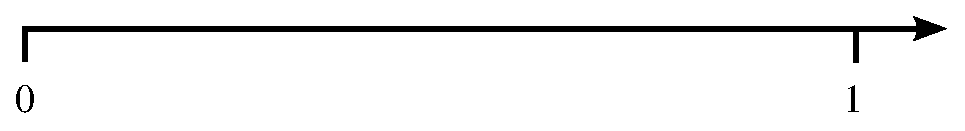
\includegraphics[width=10cm]{eps/interval.eps}
    \caption{The reference interval.}
    \label{fig:interval}
  \end{center}
\end{figure}

\begin{table}
\linespread{1.2}\selectfont
  \begin{center}
    \begin{tabular}{|c|c|}
      \hline
      Vertex & Coordinate \\
      \hline
      \hline
      $v_0$ & $x = 0$ \\
      \hline
      $v_1$ & $x = 1$ \\
      \hline
    \end{tabular}
    \caption{Vertex coordinates of the reference interval.}
    \label{tab:interval,vertices}
  \end{center}
\end{table}

\section{The reference triangle}
\index{triangle}

The reference triangle is shown in Figure~\ref{fig:triangle} and is
defined by its three vertices with coordinates as specified in
Table~\ref{tab:triangle,vertices}.

\begin{figure}
  \begin{center}
    \psfrag{v0}{$(0, 0)$}
    \psfrag{v1}{$(1, 0)$}
    \psfrag{v2}{$(0, 1)$}
    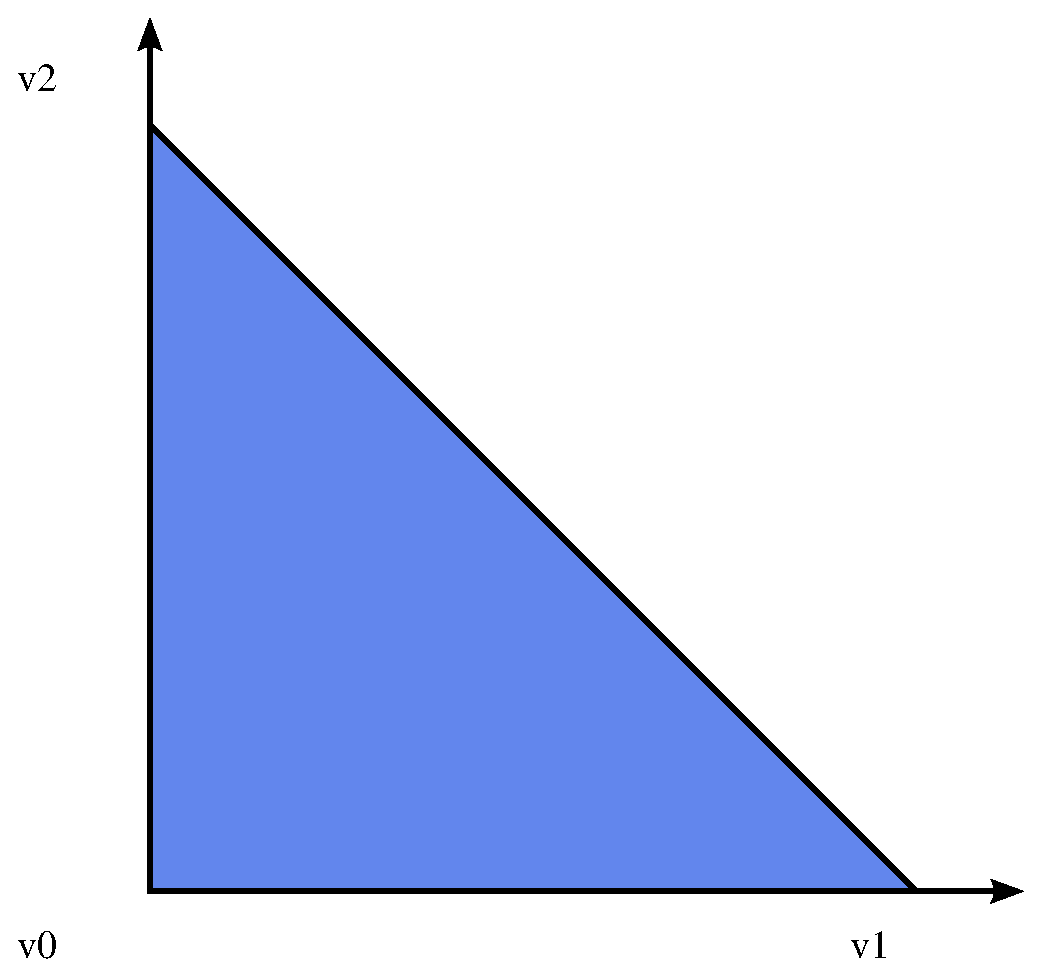
\includegraphics[width=8cm]{eps/triangle.eps}
    \caption{The reference triangle.}
    \label{fig:triangle}
  \end{center}
\end{figure}

\begin{table}
\linespread{1.2}\selectfont
  \begin{center}
    \begin{tabular}{|c|c|}
      \hline
      Vertex & Coordinate \\
      \hline
      \hline
      $v_0$ & $x = (0, 0)$ \\
      \hline
      $v_1$ & $x = (1, 0)$ \\
      \hline
      $v_2$ & $x = (0, 1)$ \\
      \hline
    \end{tabular}
    \caption{Vertex coordinates of the reference triangle.}
    \label{tab:triangle,vertices}
  \end{center}
\end{table}

\section{The reference quadrilateral}
\index{quadrilateral}

The reference quadrilateral is shown in Figure~\ref{fig:quadrilateral}
and is defined by its four vertices with coordinates as specified in
Table~\ref{tab:quadrilateral,vertices}.

\begin{figure}
  \begin{center}
    \psfrag{v0}{$(0, 0)$}
    \psfrag{v1}{$(1, 0)$}
    \psfrag{v2}{$(1, 1)$}
    \psfrag{v3}{$(0, 1)$}
    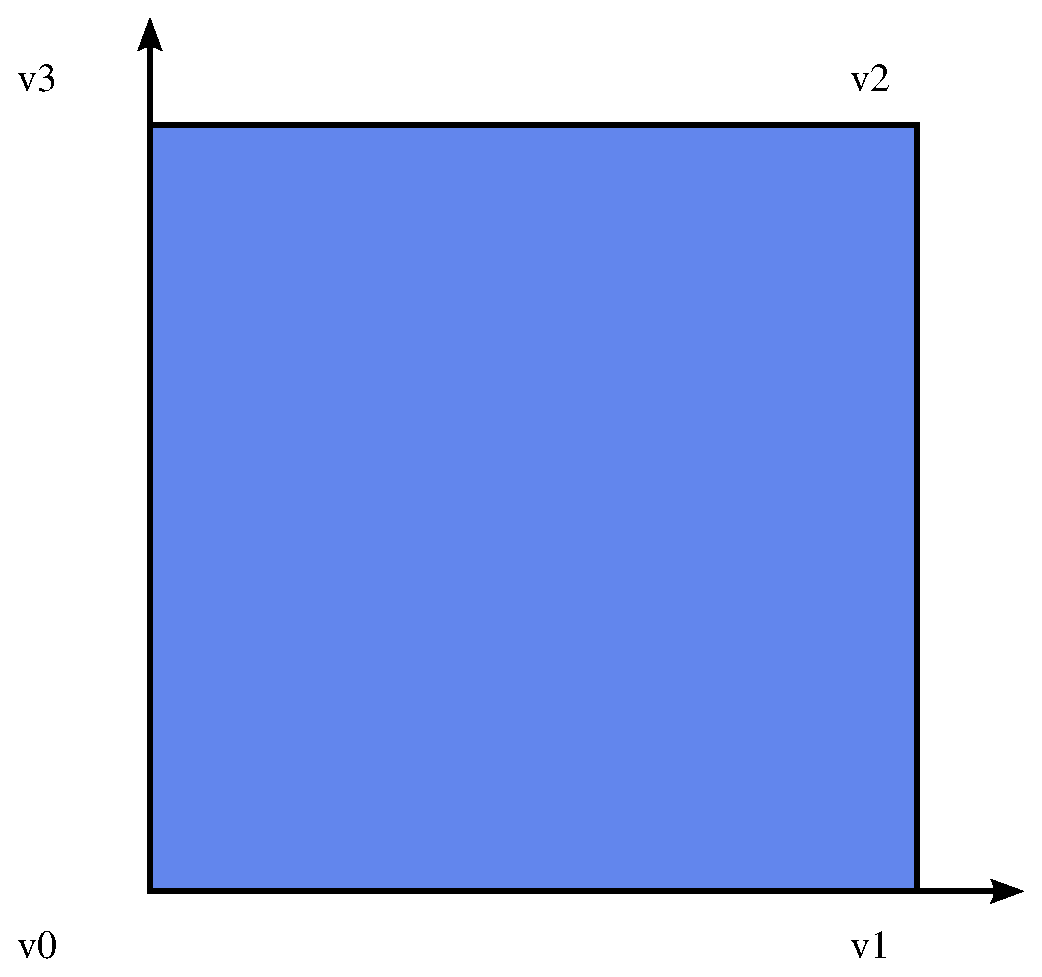
\includegraphics[width=8cm]{eps/quadrilateral.eps}
    \caption{The reference quadrilateral.}
    \label{fig:quadrilateral}
  \end{center}
\end{figure}

\begin{table}
\linespread{1.2}\selectfont
  \begin{center}
    \begin{tabular}{|c|c|}
      \hline
      Vertex & Coordinate \\
      \hline
      \hline
      $v_0$ & $x = (0, 0)$ \\
      \hline
      $v_1$ & $x = (1, 0)$ \\
      \hline
      $v_2$ & $x = (1, 1)$ \\
      \hline
      $v_3$ & $x = (0, 1)$ \\
      \hline
    \end{tabular}
    \caption{Vertex coordinates of the reference quadrilateral.}
    \label{tab:quadrilateral,vertices}
  \end{center}
\end{table}

\section{The reference tetrahedron}
\index{tetrahedron}

The reference tetrahedron is shown in Figure~\ref{fig:tetrahedron} and
is defined by its four vertices with coordinates as specified in
Table~\ref{tab:tetrahedron,vertices}.

\begin{figure}
  \begin{center}
    \psfrag{v0}{$(0, 0, 0)$}
    \psfrag{v1}{$(1, 0, 0)$}
    \psfrag{v2}{$(0, 1, 0)$}
    \psfrag{v3}{$(0, 0, 1)$}
    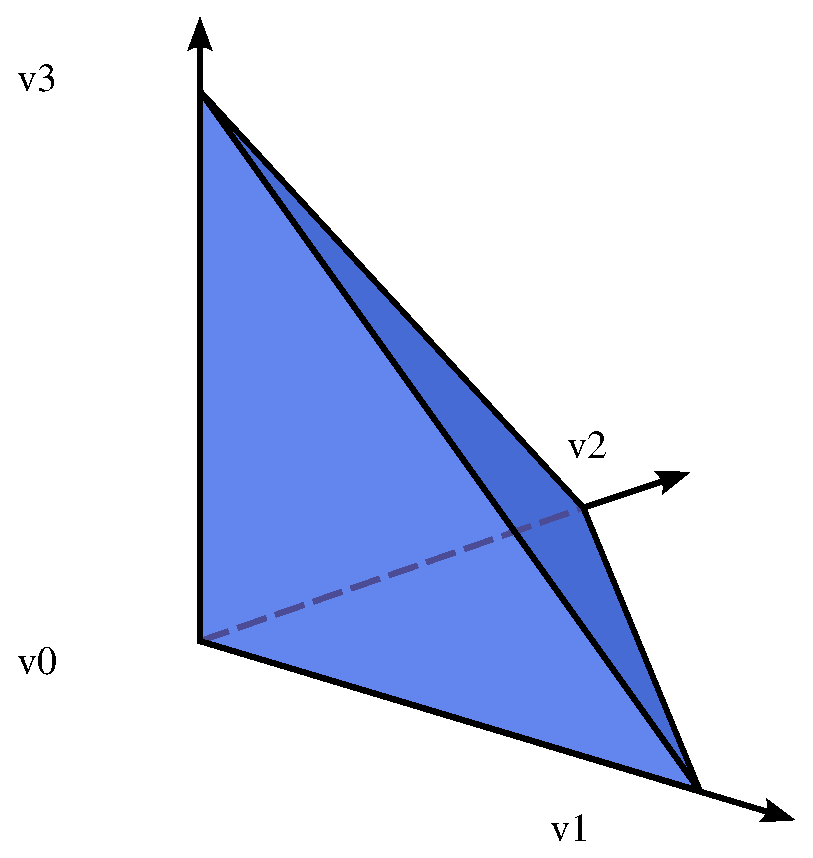
\includegraphics[width=6cm]{eps/tetrahedron.eps}
    \caption{The reference tetrahedron.}
    \label{fig:tetrahedron}
  \end{center}
\end{figure}

\begin{table}
\linespread{1.2}\selectfont
  \begin{center}
    \begin{tabular}{|c|c|}
      \hline
      Vertex & Coordinate \\
      \hline
      \hline
      $v_0$ & $x = (0, 0, 0)$ \\
      \hline
      $v_1$ & $x = (1, 0, 0)$ \\
      \hline
      $v_2$ & $x = (0, 1, 0)$ \\
      \hline
      $v_3$ & $x = (0, 0, 1)$ \\
      \hline
    \end{tabular}
    \caption{Vertex coordinates of the reference tetrahedron.}
    \label{tab:tetrahedron,vertices}
  \end{center}
\end{table}

\section{The reference hexahedron}
\index{hexahedron}

The reference hexahedron is shown in Figure~\ref{fig:hexahedron} and
is defined by its eight vertices with coordinates as specified in
Table~\ref{tab:hexahedron,vertices}.

\begin{figure}
\linespread{1.2}\selectfont
  \begin{center}
    \psfrag{v0}{$(0, 0, 0)$}
    \psfrag{v1}{$(1, 0, 0)$}
    \psfrag{v2}{$(1, 1, 0)$}
    \psfrag{v3}{$(0, 1, 0)$}
    \psfrag{v4}{$(0, 0, 1)$}
    \psfrag{v5}{$(1, 0, 1)$}
    \psfrag{v6}{$(1, 1, 1)$}
    \psfrag{v7}{$(0, 1, 1)$}
    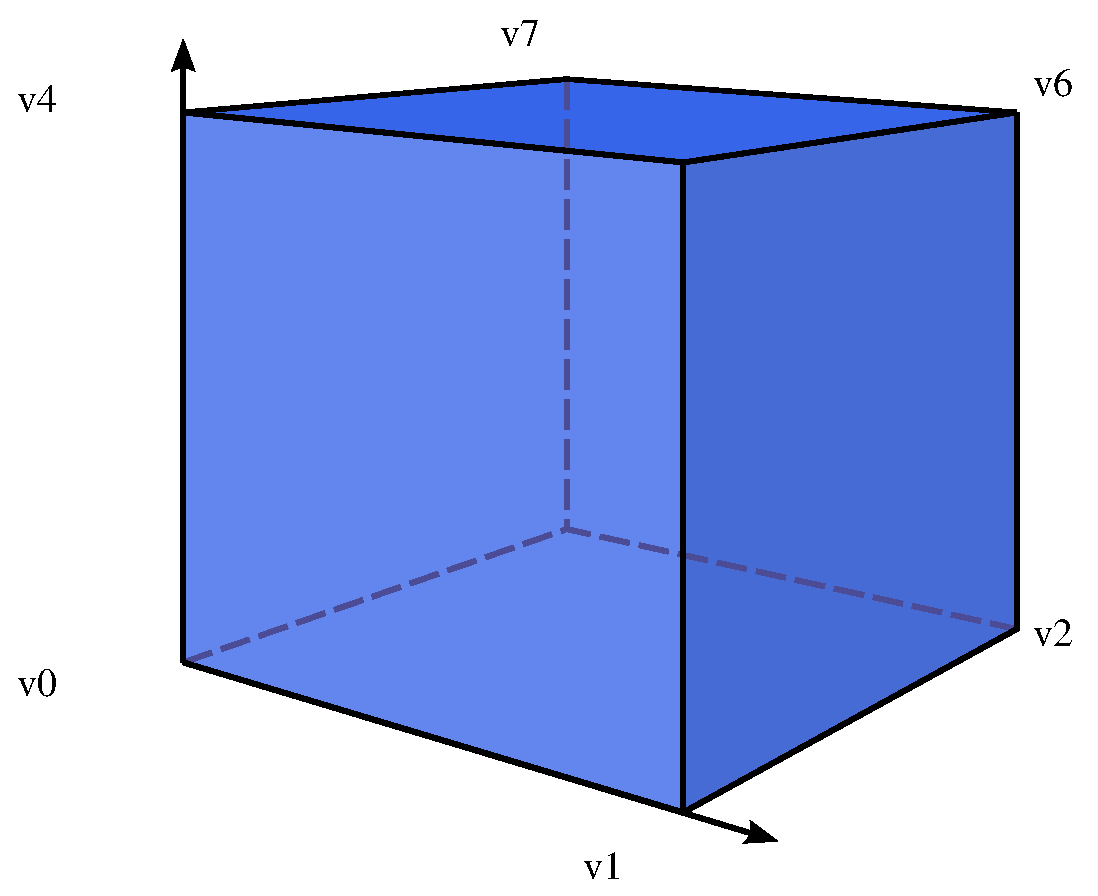
\includegraphics[width=9cm]{eps/hexahedron.eps}
    \caption{The reference hexahedron.}
    \label{fig:hexahedron}
  \end{center}
\end{figure}

\begin{table}
\linespread{1.2}\selectfont
  \begin{center}
    \begin{tabular}{|c|c|}
      \hline
      Vertex & Coordinate \\
      \hline
      \hline
      $v_0$ & $x = (0, 0, 0)$ \\
      \hline
      $v_1$ & $x = (1, 0, 0)$ \\
      \hline
      $v_2$ & $x = (1, 1, 0)$ \\
      \hline
      $v_3$ & $x = (0, 1, 0)$ \\
      \hline
    \end{tabular}
    \begin{tabular}{|c|c|}
      \hline
      Vertex & Coordinate \\
      \hline
      \hline
      $v_4$ & $x = (0, 0, 1)$ \\
      \hline
      $v_5$ & $x = (1, 0, 1)$ \\
      \hline
      $v_6$ & $x = (1, 1, 1)$ \\
      \hline
      $v_7$ & $x = (0, 1, 1)$ \\
      \hline
    \end{tabular}
    \caption{Vertex coordinates of the reference hexahedron.}
    \label{tab:hexahedron,vertices}
  \end{center}
\end{table}


\chapter{Numbering of mesh entities}

The numbering of mesh entities used in DOLFIN follows the
UFC specification.~\cite{www:UFC}
The UFC specification dictates a certain ordering of the vertices,
edges etc. of the cells of a finite element mesh. First, an \emph{ad
hoc} ordering is picked for the vertices of each cell. Then, the
remaining entities are ordered based on a simple rule, as described in
detail below.

\section{Basic concepts}

The topological entities of a cell (or mesh) are referred to as
\emph{mesh entities}. A mesh entity can be identified by a pair
$(d, i)$, where $d$ is the topological dimension of the mesh entity and $i$
is a unique index of the mesh entity. Mesh entities are numbered
within each topological dimension from $0$ to $n_d-1$, where $n_d$ is
the number of mesh entities of topological dimension $d$.

For convenience, mesh entities of topological dimension $0$ are
referred to as \emph{vertices}, entities of dimension $1$
as \emph{edges}, entities of dimension $2$ as \emph{faces}, entities of
\emph{codimension} $1$ as \emph{facets} and entities of codimension
$0$ as \emph{cells}. These concepts are summarized in
Table~\ref{tab:entities}.

Thus, the vertices of a tetrahedron are identified as
$v_0 = (0, 0)$, $v_1 = (0, 1)$ and $v_2 = (0, 2)$,
the edges are
$e_0 = (1, 0)$, $e_1 = (1, 1)$, $e_2 = (1, 2)$,
$e_3 = (1, 3)$, $e_4 = (1, 4)$ and $e_5 = (1, 5)$,
the faces (facets) are
$f_0 = (2, 0)$, $f_1 = (2, 1)$, $f_2 = (2, 2)$ and $f_3 = (2, 3)$,
and the cell itself is
$c_0 = (3, 0)$.

\begin{table}[H]
\linespread{1.2}\selectfont
  \begin{center}
    \begin{tabular}{|l|c|c|}
      \hline
      Entity & Dimension & Codimension \\
      \hline
      Vertex & $0$       & -- \\
      Edge   & $1$       & -- \\
      Face   & $2$       & -- \\
      & & \\
      Facet  & --      &  $1$ \\
      Cell   & --      &  $0$ \\
      \hline
    \end{tabular}
    \caption{Named mesh entities.}
    \label{tab:entities}
  \end{center}
\end{table}

\section{Numbering of vertices}

For simplicial cells (intervals, triangles and tetrahedra) of a finite
element mesh, the vertices are numbered locally based on the
corresponding global vertex numbers. In particular, a tuple of
increasing local vertex numbers corresponds to a tuple of increasing
global vertex numbers.  This is illustrated in
Figure~\ref{fig:numbering_example_triangles} for a mesh consisting of
two triangles.
 
\begin{figure}[htbp]
  \begin{center}
    \psfrag{v0}{$v_0$}
    \psfrag{v1}{$v_1$}
    \psfrag{v2}{$v_2$}
    \psfrag{0}{$0$}
    \psfrag{1}{$1$}
    \psfrag{2}{$2$}
    \psfrag{3}{$3$}
    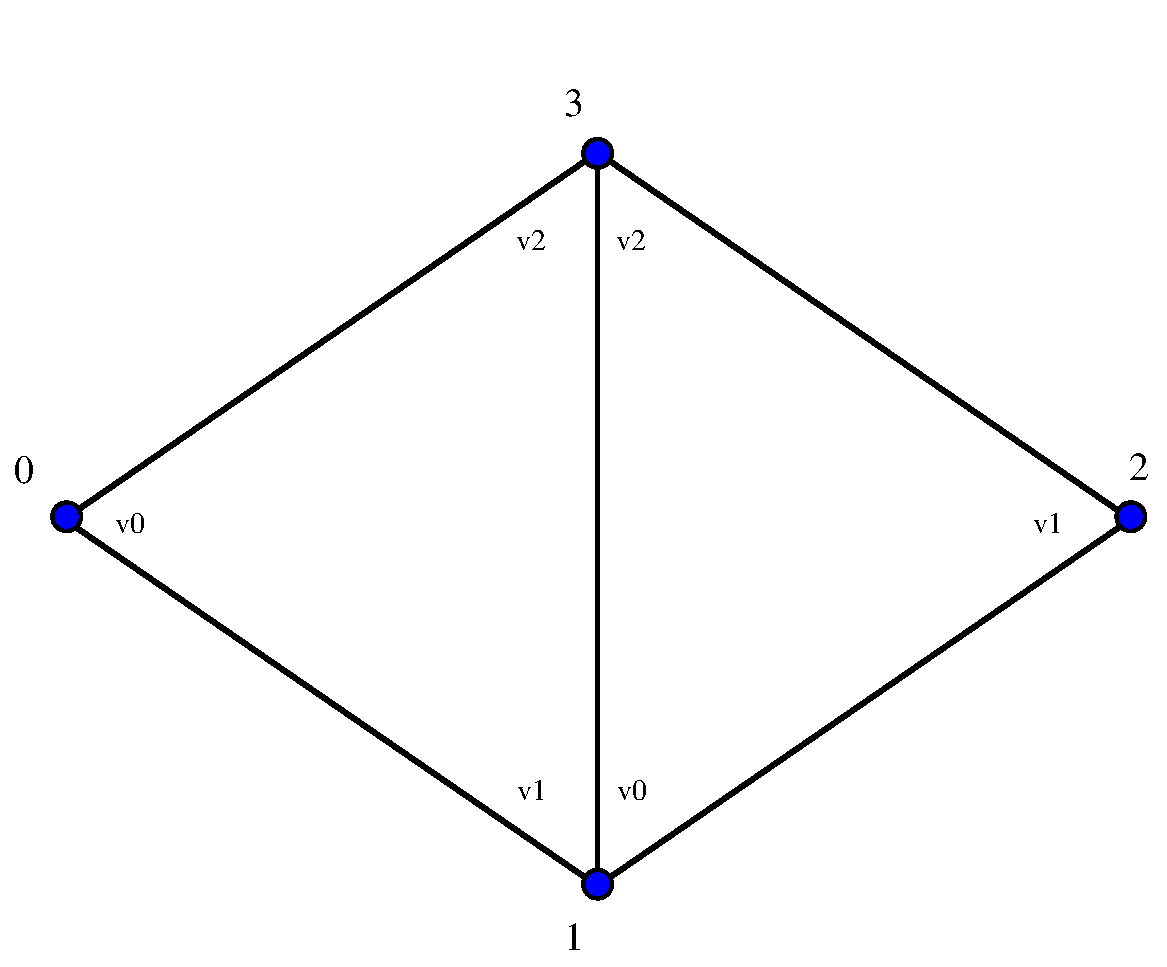
\includegraphics[width=8cm]{eps/numbering_example_triangles.eps}
    \caption{The vertices of a simplicial mesh are numbered locally
      based on the corresponding global vertex numbers.}
    \label{fig:numbering_example_triangles}
  \end{center}
\end{figure}

For non-simplicial cells (quadrilaterals and hexahedra), the ordering
is arbitrary, as long as each cell is isomorphic to the corresponding
reference cell by matching each vertex with the corresponding vertex
in the reference cell. This is illustrated in
Figure~\ref{fig:numbering_example_quadrilaterals} for a mesh
consisting of two quadrilaterals.

\begin{figure}[htbp]
  \begin{center}
    \psfrag{v0}{$v_0$}
    \psfrag{v1}{$v_1$}
    \psfrag{v2}{$v_2$}
    \psfrag{v3}{$v_3$}
    \psfrag{0}{$0$}
    \psfrag{1}{$1$}
    \psfrag{2}{$2$}
    \psfrag{3}{$3$}
    \psfrag{4}{$4$}
    \psfrag{5}{$5$}
    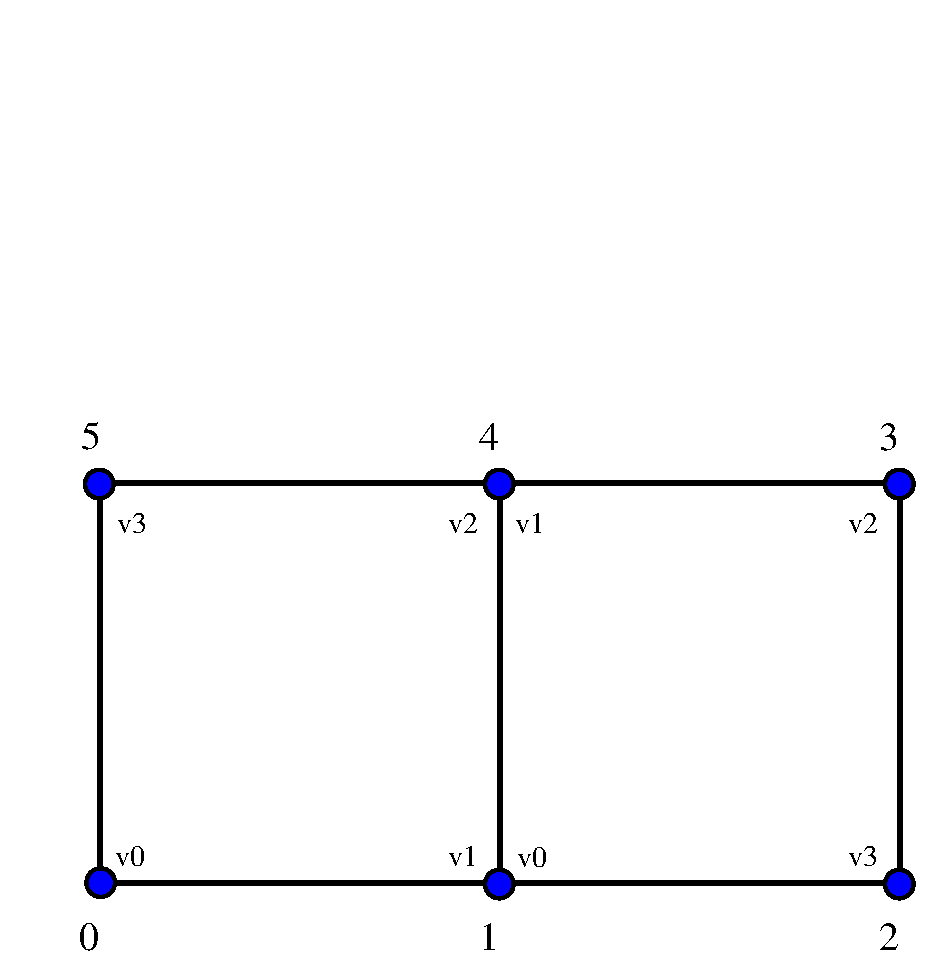
\includegraphics[width=8cm]{eps/numbering_example_quadrilaterals.eps}
    \caption{The local numbering of vertices of a non-simplicial mesh
      is arbitrary, as long as each cell is isomorphic to the
      reference cell by matching each vertex to the corresponding
      vertex of the reference cell.}
    \label{fig:numbering_example_quadrilaterals}
  \end{center}
\end{figure}

\section{Numbering of remaining mesh entities}

When the vertices have been numbered, the remaining mesh entities are
numbered within each topological dimension based on a
\emph{lexicographical ordering} of the corresponding ordered tuples of
\emph{non-incident vertices}.

As an illustration, consider the numbering of edges (the mesh entities
of topological dimension one) on the reference triangle in
Figure~\ref{fig:orderingexample,triangle}. To number the edges of the
reference triangle, we identify for each edge the corresponding
non-incident vertices. For each edge, there is only one such vertex
(the vertex opposite to the edge). We thus identify the three edges in
the reference triangle with the tuples $(v_0)$, $(v_1)$ and $(v_2)$. The
first of these is edge $e_0$ between vertices $v_1$ and $v_2$ opposite
to vertex $v_0$, the second is edge $e_1$ between vertices $v_0$ and
$v_2$ opposite to vertex $v_1$, and the third is edge $e_2$ between
vertices $v_0$ and $v_1$ opposite to vertex $v_2$.

Similarly, we identify the six edges of the reference tetrahedron with
the corresponding non-incident tuples $(v_0, v_1)$, $(v_0, v_2)$,
$(v_0, v_3)$, $(v_1, v_2)$, $(v_1, v_3)$ and $(v_2, v_3)$. The first of these is
edge $e_0$ between vertices $v_2$ and $v_3$ opposite to vertices $v_0$
and $v_1$ as shown in Figure~\ref{fig:orderingexample,tetrahedron}.

\begin{figure}[htbp]
  \begin{center}
    \psfrag{v0}{$v_0$}
    \psfrag{v1}{$v_1$}
    \psfrag{v2}{$v_2$}
    \psfrag{e0}{$e_0$}
    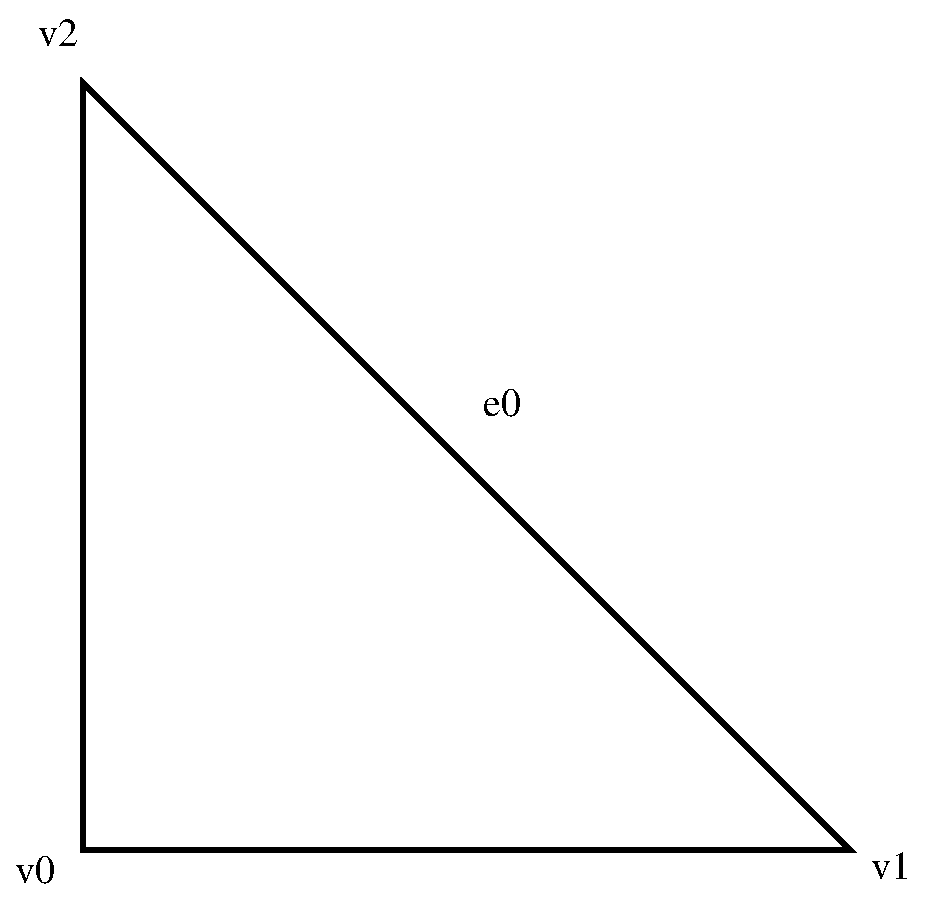
\includegraphics[width=5cm]{eps/ordering_example_triangle.eps}
    \caption{Mesh entities are ordered based on a lexicographical ordering
      of the corresponding ordered tuples of non-incident vertices.
      The first edge $e_0$ is non-incident to vertex $v_0$.}
    \label{fig:orderingexample,triangle}
  \end{center}
\end{figure}

\begin{figure}[htbp]
  \begin{center}
    \psfrag{v0}{$v_0$}
    \psfrag{v1}{$v_1$}
    \psfrag{v2}{$v_2$}
    \psfrag{v3}{$v_3$}
    \psfrag{e0}{$e_0$}
    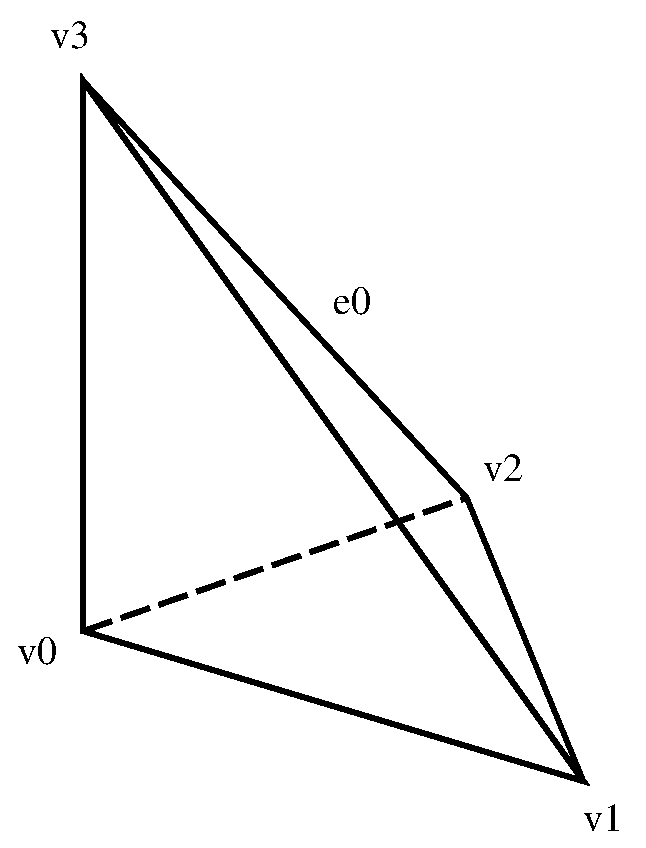
\includegraphics[width=5cm]{eps/ordering_example_tetrahedron.eps}
    \caption{Mesh entities are ordered based on a lexicographical ordering
      of the corresponding ordered tuples of non-incident vertices.
      The first edge $e_0$ is non-incident to vertices $v_0$ and $v_1$.}
    \label{fig:orderingexample,tetrahedron}
  \end{center}
\end{figure}

\subsection{Relative ordering}

The relative ordering of mesh entities with respect to other incident
mesh entities follows by sorting the entities by their (local)
indices. Thus, the pair of vertices incident to the first edge $e_0$
of a triangular cell is $(v_1, v_2)$, not $(v_2, v_1)$. Similarly, the
first face $f_0$ of a tetrahedral cell is incident to vertices $(v_1,
v_2, v_3)$.

For simplicial cells, the relative ordering in combination with the
convention of numbering the vertices locally based on global vertex
indices means that two incident cells will always agree on the
orientation of incident sub simplices. Thus, two incident triangles
will agree on the orientation of the common edge and two incident
tetrahedra will agree on the orientation of the common edge(s) and the
orientation of the common face (if any). This is illustrated in
Figure~\ref{fig:orientation_example_triangles} for two incident
triangles sharing a common edge.

\begin{figure}[htbp]
  \begin{center}
    \psfrag{v0}{$v_0$}
    \psfrag{v1}{$v_1$}
    \psfrag{v2}{$v_2$}
    \psfrag{v3}{$v_3$}
    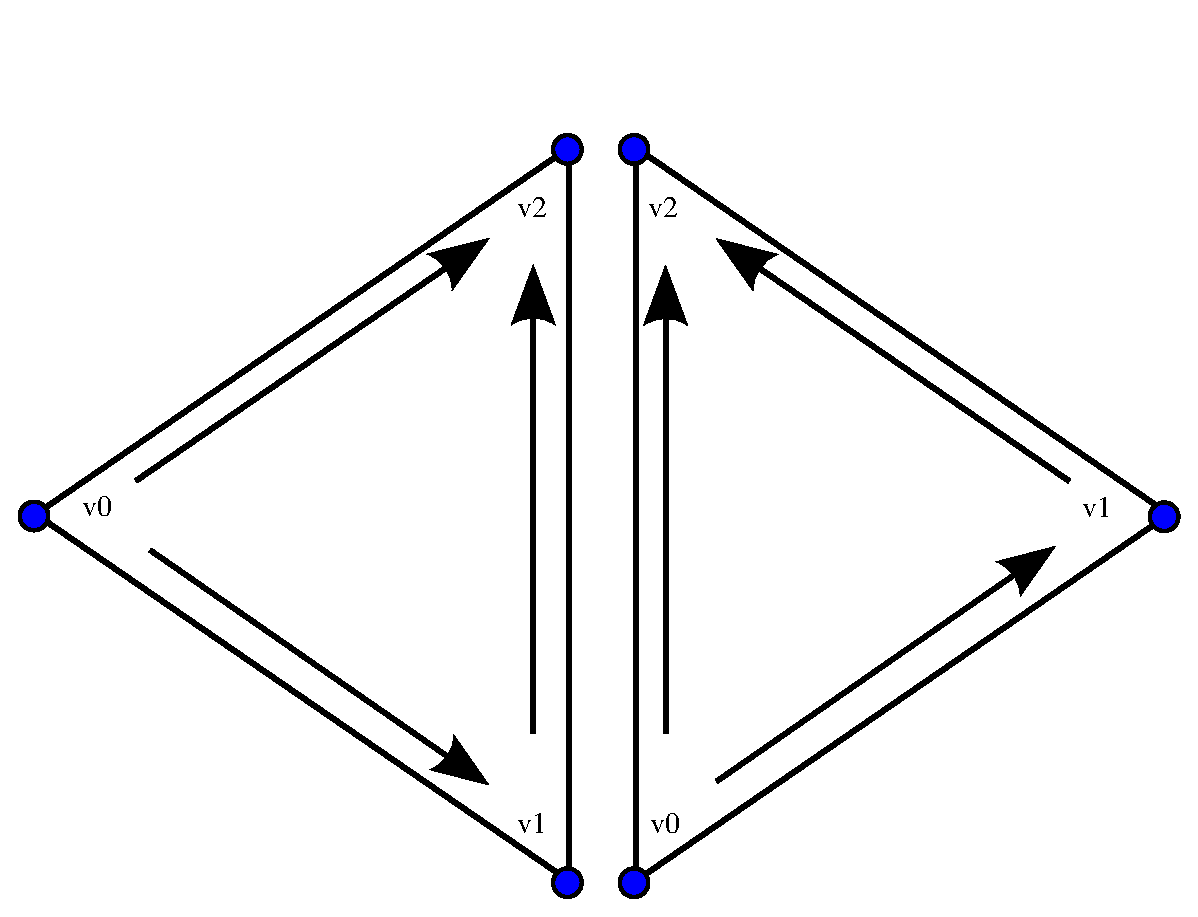
\includegraphics[width=9cm]{eps/orientation_example_triangles.eps}
    \caption{Two incident triangles will always agree on the
      orientation of the common edge.}
    \label{fig:orientation_example_triangles}
  \end{center}
\end{figure}

\subsection{Limitations}
 
The UFC specification is only concerned with the ordering of mesh
entities with respect to entities of larger topological dimension. In
other words, the UFC specification is only concerned with the ordering
of incidence relations of the class $d - d'$ where $d > d'$. For
example, the UFC specification is not concerned with the ordering of
incidence relations of the class $0 - 1$, that is, the ordering of
edges incident to vertices.

\newpage

\section{Numbering for reference cells}

The numbering scheme is demonstrated below for cells
isomorphic to each of the five reference cells.

\subsection{Numbering for intervals}

\begin{table}[H]
\linespread{1.2}\selectfont
  \begin{center}
    \begin{tabular}{|c|c|c|}
      \hline
      Entity & Incident vertices & Non-incident vertices \\
      \hline
      \hline
      $v_0 = (0, 0)$ & $(v_0)$ & $(v_1)$ \\
      \hline
      $v_1 = (0, 1)$ & $(v_1)$ & $(v_0)$ \\
      \hline
      $c_0 = (1, 0)$ & $(v_0, v_1)$ & $\emptyset$ \\
      \hline
    \end{tabular}
    \caption{Numbering of mesh entities on intervals.}
    \label{tab:interval,entities}
  \end{center}
\end{table}

\subsection{Numbering for triangular cells}

\begin{table}[H]
\linespread{1.2}\selectfont
  \begin{center}
    \begin{tabular}{|c|c|c|}
      \hline
      Entity & Incident vertices & Non-incident vertices \\
      \hline
      \hline
      $v_0 = (0, 0)$ & $(v_0)$ & $(v_1, v_2)$ \\
      \hline
      $v_1 = (0, 1)$ & $(v_1)$ & $(v_0, v_2)$ \\
      \hline
      $v_2 = (0, 2)$ & $(v_2)$ & $(v_0, v_1)$ \\
      \hline
      $e_0 = (1, 0)$ & $(v_1, v_2)$ & $(v_0)$ \\
      \hline
      $e_1 = (1, 1)$ & $(v_0, v_2)$ & $(v_1)$ \\
      \hline
      $e_2 = (1, 2)$ & $(v_0, v_1)$ & $(v_2)$ \\
      \hline
      $c_0 = (2, 0)$ & $(v_0, v_1, v_2)$ & $\emptyset$ \\
      \hline
    \end{tabular}
    \caption{Numbering of mesh entities on triangular cells.}
    \label{tab:triangle,entities}
  \end{center}
\end{table}

\subsection{Numbering for quadrilateral cells}

\begin{table}[H]
\linespread{1.1}\selectfont
  \begin{center}
    \begin{tabular}{|c|c|c|}
      \hline
      Entity & Incident vertices & Non-incident vertices \\
      \hline
      \hline
      $v_0 = (0, 0)$ & $(v_0)$ & $(v_1, v_2, v_3)$ \\
      \hline
      $v_1 = (0, 1)$ & $(v_1)$ & $(v_0, v_2, v_3)$ \\
      \hline
      $v_2 = (0, 2)$ & $(v_2)$ & $(v_0, v_1, v_3)$ \\
      \hline
      $v_3 = (0, 3)$ & $(v_3)$ & $(v_0, v_1, v_2)$ \\
      \hline
      $e_0 = (1, 0)$ & $(v_2, v_3)$ & $(v_0, v_1)$ \\
      \hline
      $e_1 = (1, 1)$ & $(v_1, v_2)$ & $(v_0, v_3)$ \\
      \hline
      $e_2 = (1, 2)$ & $(v_0, v_3)$ & $(v_1, v_2)$ \\
      \hline
      $e_3 = (1, 3)$ & $(v_0, v_1)$ & $(v_2, v_3)$ \\
      \hline
      $c_0 = (2, 0)$ & $(v_0, v_1, v_2, v_3)$ & $\emptyset$ \\
      \hline
    \end{tabular}
    \caption{Numbering of mesh entities on quadrilateral cells.}
    \label{tab:quadrilateral,entities}
  \end{center}
\end{table}

\newpage

\subsection{Numbering for tetrahedral cells}

\begin{table}[H]
\linespread{1.1}\selectfont
  \begin{center}
    \begin{tabular}{|c|c|c|}
      \hline
      Entity & Incident vertices & Non-incident vertices \\
      \hline
      \hline
      $v_0 = (0, 0)$ & $(v_0)$ & $(v_1, v_2, v_3)$ \\
      \hline
      $v_1 = (0, 1)$ & $(v_1)$ & $(v_0, v_2, v_3)$ \\
      \hline
      $v_2 = (0, 2)$ & $(v_2)$ & $(v_0, v_1, v_3)$ \\
      \hline
      $v_3 = (0, 3)$ & $(v_3)$ & $(v_0, v_1, v_2)$ \\
      \hline
      $e_0 = (1, 0)$ & $(v_2, v_3)$ & $(v_0, v_1)$ \\
      \hline
      $e_1 = (1, 1)$ & $(v_1, v_3)$ & $(v_0, v_2)$ \\
      \hline
      $e_2 = (1, 2)$ & $(v_1, v_2)$ & $(v_0, v_3)$ \\
      \hline
      $e_3 = (1, 3)$ & $(v_0, v_3)$ & $(v_1, v_2)$ \\
      \hline
      $e_4 = (1, 4)$ & $(v_0, v_2)$ & $(v_1, v_3)$ \\
      \hline
      $e_5 = (1, 5)$ & $(v_0, v_1)$ & $(v_2, v_3)$ \\
      \hline
      $f_0 = (2, 0)$ & $(v_1, v_2, v_3)$ & $(v_0)$ \\
      \hline
      $f_1 = (2, 1)$ & $(v_0, v_2, v_3)$ & $(v_1)$ \\
      \hline
      $f_2 = (2, 2)$ & $(v_0, v_1, v_3)$ & $(v_2)$ \\
      \hline
      $f_3 = (2, 3)$ & $(v_0, v_1, v_2)$ & $(v_3)$ \\
      \hline
      $c_0 = (3, 0)$ & $(v_0, v_1, v_2, v_3)$ & $\emptyset$ \\
      \hline
    \end{tabular}
    \caption{Numbering of mesh entities on tetrahedral cells.}
        \label{tab:tetrahedron,entities} 
  \end{center}
\end{table}

\vfill

\newpage

\subsection{Numbering for hexahedral cells}

\vspace{-0.5cm}
\begin{table}[H]
\small
\linespread{1.2}\selectfont
  \begin{center}
    \begin{tabular}{|c|c|c|}
      \hline
      Entity & Incident vertices & Non-incident vertices \\
      \hline
      \hline
      $v_0 = (0, 0)$ & $(v_0)$ & $(v_1, v_2, v_3, v_4, v_5, v_6, v_7)$ \\
      \hline
      $v_1 = (0, 1)$ & $(v_1)$ & $(v_0, v_2, v_3, v_4, v_5, v_6, v_7)$ \\
      \hline
      $v_2 = (0, 2)$ & $(v_2)$ & $(v_0, v_1, v_3, v_4, v_5, v_6, v_7)$ \\
      \hline
      $v_3 = (0, 3)$ & $(v_3)$ & $(v_0, v_1, v_2, v_4, v_5, v_6, v_7)$ \\
      \hline
      $v_4 = (0, 4)$ & $(v_4)$ & $(v_0, v_1, v_2, v_3, v_5, v_6, v_7)$ \\
      \hline
      $v_5 = (0, 5)$ & $(v_5)$ & $(v_0, v_1, v_2, v_3, v_4, v_6, v_7)$ \\
      \hline
      $v_6 = (0, 6)$ & $(v_6)$ & $(v_0, v_1, v_2, v_3, v_4, v_5, v_7)$ \\
      \hline
      $v_7 = (0, 7)$ & $(v_7)$ & $(v_0, v_1, v_2, v_3, v_4, v_5, v_6)$ \\
      \hline
      $e_0 = (1, 0)$ & $(v_6, v_7)$ & $(v_0, v_1, v_2, v_3, v_4, v_5)$ \\
      \hline
      $e_1 = (1, 1)$ & $(v_5, v_6)$ & $(v_0, v_1, v_2, v_3, v_4, v_7)$ \\
      \hline
      $e_2 = (1, 2)$ & $(v_4, v_7)$ & $(v_0, v_1, v_2, v_3, v_5, v_6)$ \\
      \hline
      $e_3 = (1, 3)$ & $(v_4, v_5)$ & $(v_0, v_1, v_2, v_3, v_6, v_7)$ \\
      \hline
      $e_4 = (1, 4)$ & $(v_3, v_7)$ & $(v_0, v_1, v_2, v_4, v_5, v_6)$ \\
      \hline
      $e_5 = (1, 5)$ & $(v_2, v_6)$ & $(v_0, v_1, v_3, v_4, v_5, v_7)$ \\
      \hline
      $e_6 = (1, 6)$ & $(v_2, v_3)$ & $(v_0, v_1, v_4, v_5, v_6, v_7)$ \\
      \hline
      $e_7 = (1, 7)$ & $(v_1, v_5)$ & $(v_0, v_2, v_3, v_4, v_6, v_7)$ \\
      \hline
      $e_8 = (1, 8)$ & $(v_1, v_2)$ & $(v_0, v_3, v_4, v_5, v_6, v_7)$ \\
      \hline
      $e_9 = (1, 9)$ & $(v_0, v_4)$ & $(v_1, v_2, v_3, v_5, v_6, v_7)$ \\
      \hline
      $e_{10} = (1, 10)$ & $(v_0, v_3)$ & $(v_1, v_2, v_4, v_5, v_6, v_7)$ \\
      \hline
      $e_{11} = (1, 11)$ & $(v_0, v_1)$ & $(v_2, v_3, v_4, v_5, v_6, v_7)$ \\
      \hline
      $f_0 = (2, 0)$ & $(v_4, v_5, v_6, v_7)$ & $(v_0, v_1, v_2, v_3)$ \\
      \hline
      $f_1 = (2, 1)$ & $(v_2, v_3, v_6, v_7)$ & $(v_0, v_1, v_4, v_5)$ \\
      \hline
      $f_2 = (2, 2)$ & $(v_1, v_2, v_5, v_6)$ & $(v_0, v_3, v_4, v_7)$ \\
      \hline
      $f_3 = (2, 3)$ & $(v_0, v_3, v_4, v_7)$ & $(v_1, v_2, v_5, v_6)$ \\
      \hline
      $f_4 = (2, 4)$ & $(v_0, v_1, v_4, v_5)$ & $(v_2, v_3, v_6, v_7)$ \\
      \hline
      $f_5 = (2, 5)$ & $(v_0, v_1, v_2, v_3)$ & $(v_4, v_5, v_6, v_7)$ \\
      \hline
      $c_0 = (3, 0)$ & $(v_0, v_1, v_2, v_3, v_4, v_5, v_6, v_7)$ & $\emptyset$ \\
      \hline
    \end{tabular}
    \caption{Numbering of mesh entities on hexahedral cells.}
    \label{tab:hexahedron,entities}
  \end{center}
\end{table}


\chapter{Design}

This chapter discusses details of the design of \dolfin{} and is
intended mainly for developers of \dolfin{}.

\section{Linear algebra}

The linear algebra library provides a uniform interface to uBlas
and PETSc linear algebra through a set of wrappers for basic data
structures (matrices and vectors) and solvers, such as Krylov subspace
solvers with preconditioners.

For both sets of wrappers, a common interface is defined by the
classes \texttt{GenericMatrix} and \texttt{GenericVector}. \dolfin{}
provides a number of algorithms, most notably the assembly algorithms,
that work only through the common interface, which means that these
algorithms work for any given representation that implements the
interface specified by \texttt{GenericMatrix} or
\texttt{GenericVector}. A class diagram for the \dolfin{} linear
algebra implementation is given in Figure~\ref{fig:laclasses}.

\begin{figure}[htbp]
  \begin{center}
    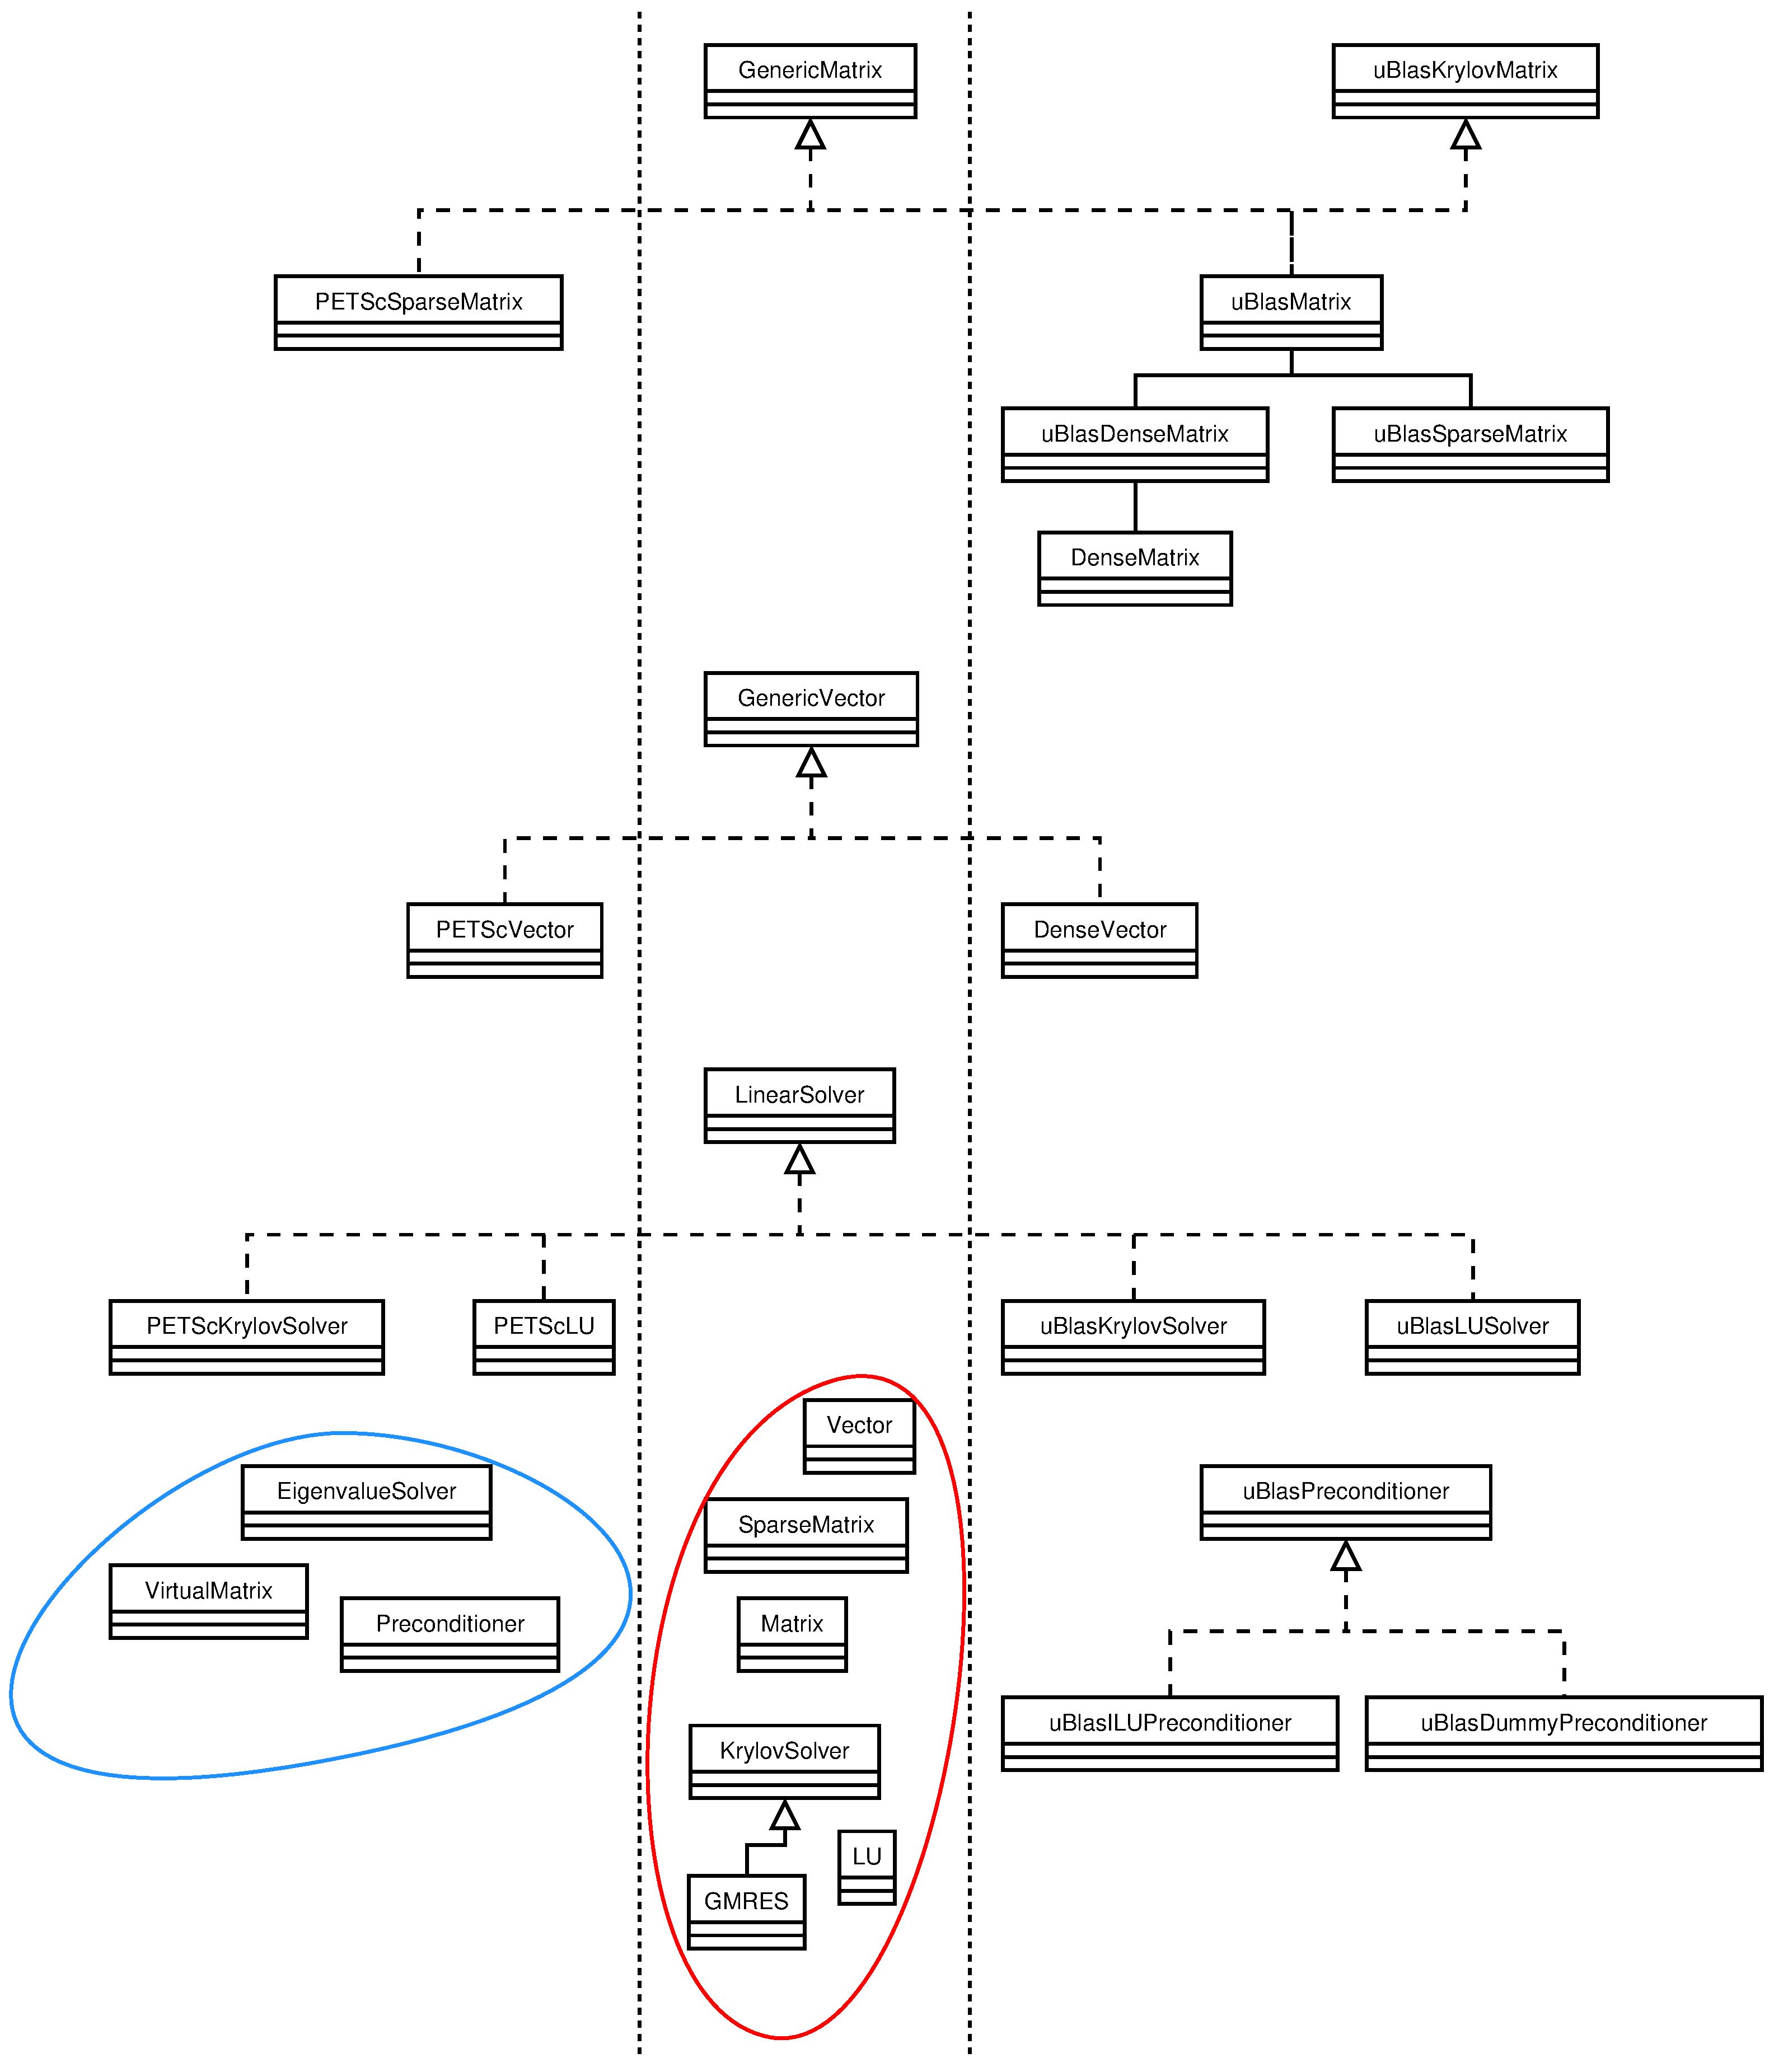
\includegraphics[width=0.95\textwidth]{eps/class-diagram-la.eps}
    \caption{Class diagram of the linear algebra classes in \dolfin{}.}
    \label{fig:laclasses}
  \end{center}
\end{figure}


\chapter{Installation}
\index{installation}

The source code of \dolfin{} is portable and should compile on any
Unix system, although it is developed mainly under GNU/Linux
(in particular Debian GNU/Linux). Questions, bug reports and patches
concerning the installation should be directed to the
\dolfin{} mailing list at the address
\begin{code}
  dolfin-dev@fenics.org
\end{code}

\dolfin{} must currently be compiled directly from source, but effort
is underway to provide precompiled Debian packages of \dolfin{} and
other \fenics{} components.

%------------------------------------------------------------------------------
\section{Installing from source}

\subsection{Dependencies and requirements}
\index{dependencies}

\dolfin{} depends on a number of libraries that need to be installed on your
system. These libraries include Libxml2 and PETSc. In addition to these libraries,
you need to install \fiat{} and \ffc{} if you want to define your own variational forms.

\subsubsection{Installing Libxml2}
\index{Libxml2}

Libxml2 is a library used by \dolfin{} to parse XML data files. Libxml2 can be obtained from
\begin{code}
  http://xmlsoft.org/
\end{code}
For Debian users, the package to install is \texttt{libxml2-dev}.

\subsubsection{Installing PETSc}
\index{PETSc}

PETSc is a library for the solution of linear and nonlinear systems, functioning as the backend
for the \dolfin{} linear algebra classes. \dolfin{} depends on PETSc version 2.3.0, which can be
obtained from
\begin{code}
  http://www-unix.mcs.anl.gov/petsc/petsc-2/
\end{code}

Follow the installation instructions on the PETSc web page. Normally,
you should only have to perform the following simple steps in the PETSc
source directory:
\begin{code}
  # export PETSC_DIR=`pwd`
  # ./config/configure.py --with-clanguage=cxx --with-shared=1
  # make all
\end{code}

Add \texttt{--download-hypre=yes} to configure.py if you want to
install Hypre which provides a collection of preconditioners,
including algebraic multigrid (AMG).

DOLFIN assumes that \texttt{PETSC\_DIR} is
\texttt{/usr/local/lib/petsc/} but this can be controlled using the
flag \texttt{--with-petsc-dir=<path>} when configuring DOLFIN (see
below).

\subsubsection{Installing FFC}
\index{ffc}

\dolfin{} uses the FEniCS Form Compiler \ffc{} to process variational
forms. \ffc{} can be obtained from
\begin{code}
  http://www.fenics.org/
\end{code}

Follow the installation instructions given in the \ffc{}
manual. \ffc{} follows the standard for Python packages, which means
that normally you should only have to perform the following simple step
in the \ffc{} source directory:
\begin{code}
  # python setup.py install
\end{code}

Note that \ffc{} depends on \fiat{} \index{fiat}, which in turn depends on
the Python packages Numeric (Debian package \texttt{python-numeric}) and
LinearAlgebra (Debian package \texttt{python-numeric-ext}). Refer to
the \ffc{} manual for further details.

% Input section shared with FFC manual
% This chapter is common to the DOLFIN and FFC manuals.

\subsection{Downloading the source code}
\index{downloading}
\index{source code}

The latest release of \package{} can be obtained as a \texttt{tar.gz}
archive in the download section at
\begin{code}
 http://www.fenics.org/
\end{code}

Download the latest release of \package{}, for example \texttt{\packagett{}-x.y.z.tar.gz},
and unpack using the command
\begin{macrocode}
# tar zxfv \packagett{}-x.y.z.tar.gz
\end{macrocode}

This creates a directory \texttt{\packagett{}-x.y.z} containing the
\package{} source code.

If you want the very latest version of \package{}, it can be accessed
directly from the development repository through \texttt{hg}
(Mercurial):
\begin{macrocode}
# hg clone http://www.fenics.org/hg/\packagett{}
\end{macrocode}
This version may contain features not yet present in the latest
release, but may also be less stable and even not work at all.


\subsection{Compiling the source code}
\index{compiling}

\dolfin{} is built using the standard GNU Autotools (Automake,
Autoconf), which means that the installation procedure is simple:
\begin{code}
  # ./configure
  # make
\end{code}
followed by an optional
\begin{code}
  # make install
\end{code}
to install \dolfin{} on your system.

The configure script will check for a number of libraries and try
to figure out how compile \dolfin{} against these libraries. The
configure script accepts a collection of optional arguments that can be
used to control the compilation process. A few of these are listed
below. Use the command
\begin{code}
  # ./configure --help
\end{code}
for a complete list of arguments.

\begin{itemize}
\item
  Use the option \texttt{--prefix=<path>} to specify an alternative
  directory for installation of \dolfin{}. The default directory is
  \texttt{/usr/local/}, which means that header files will be
  installed under \texttt{/usr/local/inlude/} and libraries will be
  installed under \texttt{/usr/local/lib/}. This option can be useful
  if you don't have root access but want to install \dolfin{} locally
  on a user account as follows:
  \begin{code}
    # mkdir ~/local
    # ./configure --prefix=~/local
    # make
    # make install
  \end{code}
\item
  Use the option \texttt{--enable-debug} to compile \dolfin{} with
  debugging symbols and assertions.
\item
  Use the option \texttt{--enable-optimization} to compile an
  optimized version of \dolfin{} without debugging symbols
  and assertions.
\item
  Use the option \texttt{--disable-curses} to compile \dolfin{}
  without the curses interface (a text-mode graphical user interface).
\item
  Use the option \texttt{--disable-mpi} to compile \dolfin{} without
  support for MPI (Message Passing Interface), assuming PETSc has been
  compiled without support for MPI.
\item
  Use the option \texttt{--with-petsc-dir=<path>} to specify the
  location of the PETSc directory. By default, \dolfin{} assumes that
  PETSc has been installed in \texttt{/usr/local/lib/petsc/}.
\end{itemize}

\subsection{Compiling the demo programs}
\index{demo programs}

After compiling the \dolfin{} library according to the instructions
above, you may want to try one of the demo programs in the
subdirectory \texttt{src/demo/} of the \dolfin{} source tree.
Just enter the directory containing the demo program you want to
compile and type \texttt{make}. You may also compile all demo programs
at once using the command
\begin{code}
  # make demo
\end{code}

\subsection{Compiling a program against \dolfin{}}
\index{compiling}

Whether you are writing your own Makefiles or using an automated build
system such as GNU Autotools or BuildSystem, it is straightforward to
compile a program against \dolfin{}. The necessary include and library
paths can be obtained through the script \texttt{dolfin-config} which
is automatically generated during the compilation of \dolfin{} and
installed in the \texttt{bin} subdirectory of the \texttt{<path>}
specified with \texttt{--prefix}. Assuming this directory is in your
executable path (environment variable \texttt{PATH}), the include
path for building \dolfin{} can be obtained from the command
\begin{code}
  dolfin-config --cflags
\end{code}
and the path to \dolfin{} libraries can be obtained from the command
\begin{code}
  dolfin-config --libs
\end{code}
If \texttt{dolfin-config} is not in your executable path, you need to
provide the full path to \texttt{dolfin-config}.

Examples of how to write a proper \texttt{Makefile} are provided with
each of the example programs in the subdirectory \texttt{src/demo/} in
the \dolfin{} source tree.

%------------------------------------------------------------------------------
\section{Debian package}
\index{Debian package}

In preparation.

% This chapter is common to the DOLFIN and FFC manuals.

\chapter{Contributing code}
\index{contributing}

If you have created a new module, fixed a bug somewhere, or have made
a small change which you want to contribute to \package{}, then the
best way to do so is to send us your contribution in the form of a
patch. A patch is a file which describes how to transform a file or
directory structure into another. The patch is built by comparing a
version which both parties have against the modified version which
only you have.

%------------------------------------------------------------------------------
\section{Creating a patch}
\index{diff}
\index{patch}

The tool used to create a patch is called \texttt{diff} and the tool
used to apply the patch is called \texttt{patch}. These tools are free
software and are standard on most Unix systems.

Here's an example of how it works. Start from the latest release of
\package{}, which we here assume is release 0.1.0. You then have a
directory structure under \texttt{\packagett{}-0.1.0} where you have made
modifications to some files which you think could be useful to
other users.

\begin{enumerate}
\item
  Clean up your modified directory structure to remove temporary and binary
  files which will be rebuilt anyway:
  \begin{code}
# make clean
  \end{code}
\item
  From the parent directory, rename the \package{} directory to something else:
  \begin{macrocode}
# mv \packagett{}-0.1.0 \packagett{}-0.1.0-mod
  \end{macrocode}
\item
  Unpack the version of \package{} that you started from:
  \begin{macrocode}
# tar zxfv \packagett{}-0.1.0.tar.gz
  \end{macrocode}
\item
  You should now have two \package{} directory structures in your current directory:
  \begin{macrocode}
# ls
\packagett{}-0.1.0
\packagett{}-0.1.0-mod
  \end{macrocode}
\item
  Now use the \texttt{diff} tool to create the patch:
  \begin{macrocode}
# diff -u --new-file --recursive \packagett{}-0.1.0
 \packagett{}-0.1.0-mod > \packagett{}-<identifier>-<date>.patch
  \end{macrocode}
  written as one line, where \texttt{<identifier>} is a keyword that
  can be used to identify the patch as coming from you (your username,
  last name, first name, a nickname etc) and \texttt{<date>} is
  today's date in the format \texttt{yyyy-mm-dd}.
\item
  The patch now exists as \texttt{\packagett{}-<identifier>-<date>.patch}
  and can be distributed to other people who already have
  \texttt{\packagett{}-0.1.0} to easily create your modified version. If the
  patch is large, compressing it with for example \texttt{gzip} is
  advisable:
  \begin{macrocode}
# gzip \packagett{}-<identifier>-<date>.patch
  \end{macrocode}
\end{enumerate}

%------------------------------------------------------------------------------
\section{Sending patches}
\index{patch}

Patch files should be sent to the \package{} mailing list at the address
\begin{macrocode}
\packagett{}-dev@fenics.org
\end{macrocode}
Include a short description of what your patch accomplishes. Small
patches have a better chance of being accepted, so if you are making a
major contribution, please consider breaking your changes up into
several small self-contained patches if possible.

%------------------------------------------------------------------------------
\section{Applying a patch (maintainers)}
\index{patch}

Let's say that a patch has been built relative to \package{} release 0.1.0.
The following description then shows how to apply the patch to a clean
version of release 0.1.0.

\begin{enumerate}
\item
  Unpack the version of \package{} which the patch is built relative to:
  \begin{macrocode}
# tar zxfv \packagett{}-0.1.0.tar.gz
  \end{macrocode}
\item
  Check that you have the patch \texttt{\packagett{}-<identifier>-<date>.patch} and the \package{}
  directory structure in the current directory:
  \begin{macrocode}
# ls
\packagett{}-0.1.0
\packagett{}-<identifier>-<date>.patch
  \end{macrocode}
  Unpack the patch file using \texttt{gunzip} if necessary.
\item
  Enter the \package{} directory structure:
  \begin{macrocode}
# cd \packagett{}-0.1.0
  \end{macrocode}
\item
  Apply the patch:
  \begin{macrocode}
# patch -p1 < ../\packagett{}-<identifier>-<date>.patch
  \end{macrocode}
  The option \texttt{-p1} strips the leading directory from the filename
  references in the patch, to match the fact that we are applying the
  patch from inside the directory. Another useful option to
  \texttt{patch} is \texttt{--dry-run} which can be used to test the
  patch without actually applying it.
\item
  The modified version now exists as \texttt{\packagett{}-0.1.0}.
\end{enumerate}

% DOLFIN-specific part of chapter contributing.tex

%------------------------------------------------------------------------------
\section{License agreement}
\index{license}

By contributing a patch to \package{}, you agree to license your
contributed code under the GNU Lesser General Public License (a
condition also built into the LGPL license of the code you have
modified). Before creating the patch, please update the author and
date information of the file(s) you have modified according to the
following example:

\begin{code}
// Copyright (C) 2004-2005 Johan Hoffman and Anders Logg.
// Licensed under the GNU LGPL Version 2.1.
//
// Modified by Johan Jansson 2005.
// Modified by Garth N. Wells 2005.
//
// First added:  2004-06-22
// Last changed: 2005-09-01
\end{code}

As a rule of thumb, the original author of a file holds the copyright.

\chapter{Contributors}

\devnote{List all contributors here.}
\chapter{Coding style}
\label{sec:codingstyle}
\index{coding style}

To streamline the \dolfin{} source code and ease the job for
maintainers that need to read and edit large amounts of code,
developers should try to follow the below coding style when submitting
patches to \dolfin{}.

The guideline below is for C++ but may in some cases be extrapolated
to Python.

\section{Naming conventions}

\subsection{Class names}

Use camel caps for class names:
\begin{code}
class FooBar
{
  ...
};
\end{code}

\subsection{Function names}

Use lower-case for function names and underscore to separate words:
\begin{code}
void foo();
void bar();
void foo_bar(...);
\end{code}

Functions returning a value should be given the name of that value,
for example:
\begin{code}
class Array:
{
public:

  /// Return size of array (number of entries)
  uint size() const;

};
\end{code}

In the above example, the function should be named \texttt{size} rather
than \texttt{get\_size}. On the other hand, a function not returning a
value but rather taking a variable (by reference) and assigning a value
to it, should use the \texttt{get\_foo} naming scheme, for example:
\begin{code}
class Parameters:
{
public:

  /// Retrieve all parameter keys
  void get_parameter_keys(std::vector<std::string>& parameter_keys) const;

};
\end{code}

\subsection{Variable names}

Use lower-case for variable names and underscore to separate words:
\begin{code}
Foo foo;
Bar bar;
FooBar foo_bar;
\end{code}

\subsection{Enum variables and constants}

Enum variables should be lower-case with underscore to separate words:
\begin{code}
enum Type {foo, bar, foo_bar};
\end{code}

We try to avoid using \texttt{\#define} to define constants, but when
necessary constants should be capitalized:
\begin{code}
#define FOO 3.14159265358979
\end{code}

\subsection{File names}

Use camel caps for file names if they contain the
declaration/definition of a class. Header files should have the
suffix~\texttt{.h} and implementation files should have the
suffix~\texttt{.cpp}:
\begin{code}
FooBar.h
FooBar.cpp
\end{code}

Use lower-case for file names that contain utilities/functions (not
classes).

\section{Miscellaneous}

\subsection{Comments}

Comment your code, and do it often. Capitalize the first letter and
don't use punctuation (unless the comment runs over several
sentences). Here's a good example from \texttt{TopologyComputation.cpp}:
\begin{code}
// Check if connectivity has already been computed
if (connectivity.size() > 0)
  return;

// Invalidate ordering
mesh._ordered = false;

// Compute entities if they don't exist
if (topology.size(d0) == 0)
  computeEntities(mesh, d0);
if (topology.size(d1) == 0)
  computeEntities(mesh, d1);

// Check if connectivity still needs to be computed
if (connectivity.size() > 0)
  return;

...
\end{code}

\subsection{Integers and reals}

Use \texttt{dolfin::uint} instead of \texttt{int} (unless you really
want to use negative integers which is rare) and \texttt{dolfin::real}
instead of \texttt{double}:
\begin{code}
uint i = 0;
double x = 0.0;
\end{code}
These are typedefs for the standard C++ types \texttt{unsigned int}
and \texttt{double} (defined in \texttt{dolfin/common/types.h}).

\subsection{Placement of brackets}

Curly brackets following a control statement should appear in the next
line and not be indented:
\begin{code}
for (uint i = 0; i < 10; i++)
{
  ...
}
\end{code}

\subsection{Indentation}

Indentation should be two spaces and it should be spaces, \emph{not}
tab(s).

\subsection{Header file layout}

Header files should follow the below template:
\vspace{-0.5cm}
\begin{code}
// Copyright (C) 2008 Foo Bar.
// Licensed under the GNU LGPL Version 2.1.
//
// Modified by Bar Foo, 2008.
//
// First added:  2008-01-01
// Last changed: 2008-02-01

#ifndef __FOO_H
#define __FOO_H

namespace dolfin
{

  class Bar; // Forward declarations here

  /// Documentation of class

  class Foo
  {
  public:

    ...

  private:

    ...

  };

}

#endif
\end{code}

\subsection{Implementation file layout}

Implementation files should follow the below template:
\begin{code}
// Copyright (C) 2008 Foo Bar.
// Licensed under the GNU LGPL Version 2.1.
//
// Modified by Bar Foo, 2008.
//
// First added:  2008-01-01
// Last changed: 2008-02-01

#include <dolfin/Foo.h>

using namespace dolfin;

//-----------------------------------------------------------
Foo::Foo() : // variable initialization here
{
  ...
}
//-----------------------------------------------------------
Foo::~Foo()
{
  // Do nothing
}
//-----------------------------------------------------------
\end{code}

The horizontal lines above should be exactly~79 characters
wide but have been shortened here to fit the page.

\subsection{Including header files}

Don't use \texttt{\#include <dolfin.h>} or \texttt{\#include
  <dolfin/dolfin\_foo.h>} inside the DOLFIN kernel. Only include the
portions of DOLFIN you are actually using.

\subsection{Forward declarations}

Actually, try to include as little as possible and use forward
declarations whenever possible (in header files). Put the
\texttt{\#include} in the implementation file.

\subsection{Explicit constructors}

Make all constructors (except copy constructors) explicit if there is no particular
reason not to do so:
\begin{code}
class Foo
{
  explicit Foo(uint i);
};
\end{code}

\subsection{Virtual functions}

Always declare inherited virtual functions as virtual in the subclasses. This makes it
easier to spot which functions are virtual.

\begin{code}
class Foo
{
  virtual void foo();
  virtual void bar() = 0;
};

class Bar
{
  virtual void foo();
  virtual void bar();
};
\end{code}

\section{Use of libraries}

\subsection{Prefer C++ strings and streams to old C-style \texttt{char*}}

Use std::string instead of \texttt{const char*} and use std::istream and
std::ostream instead of \texttt{FILE}. Avoid \texttt{printf},
\texttt{sprintf} and the like.

There are exceptions to this rule where we need to use old C-style
function calls. One such exception is handling of command-line
arguments (\texttt{char* argv[]}).

% This chapter is common to the DOLFIN and FFC manuals.

\chapter{License}
\index{LGPL}
\index{GNU Lesser General Public License}
\index{license}

\package{} is licensed under the GNU Lesser General Public License
(LGPL) version 2.1, included verbatim below.

\footnotesize
\begin{verbatim}
		  GNU LESSER GENERAL PUBLIC LICENSE
		       Version 2.1, February 1999

 Copyright (C) 1991, 1999 Free Software Foundation, Inc.
 51 Franklin Street, Fifth Floor, Boston, MA  02110-1301  USA
 Everyone is permitted to copy and distribute verbatim copies
 of this license document, but changing it is not allowed.

[This is the first released version of the Lesser GPL.  It also counts
 as the successor of the GNU Library Public License, version 2, hence
 the version number 2.1.]

			    Preamble

  The licenses for most software are designed to take away your
freedom to share and change it.  By contrast, the GNU General Public
Licenses are intended to guarantee your freedom to share and change
free software--to make sure the software is free for all its users.

  This license, the Lesser General Public License, applies to some
specially designated software packages--typically libraries--of the
Free Software Foundation and other authors who decide to use it.  You
can use it too, but we suggest you first think carefully about whether
this license or the ordinary General Public License is the better
strategy to use in any particular case, based on the explanations below.

  When we speak of free software, we are referring to freedom of use,
not price.  Our General Public Licenses are designed to make sure that
you have the freedom to distribute copies of free software (and charge
for this service if you wish); that you receive source code or can get
it if you want it; that you can change the software and use pieces of
it in new free programs; and that you are informed that you can do
these things.

  To protect your rights, we need to make restrictions that forbid
distributors to deny you these rights or to ask you to surrender these
rights.  These restrictions translate to certain responsibilities for
you if you distribute copies of the library or if you modify it.

  For example, if you distribute copies of the library, whether gratis
or for a fee, you must give the recipients all the rights that we gave
you.  You must make sure that they, too, receive or can get the source
code.  If you link other code with the library, you must provide
complete object files to the recipients, so that they can relink them
with the library after making changes to the library and recompiling
it.  And you must show them these terms so they know their rights.

  We protect your rights with a two-step method: (1) we copyright the
library, and (2) we offer you this license, which gives you legal
permission to copy, distribute and/or modify the library.

  To protect each distributor, we want to make it very clear that
there is no warranty for the free library.  Also, if the library is
modified by someone else and passed on, the recipients should know
that what they have is not the original version, so that the original
author's reputation will not be affected by problems that might be
introduced by others.

  Finally, software patents pose a constant threat to the existence of
any free program.  We wish to make sure that a company cannot
effectively restrict the users of a free program by obtaining a
restrictive license from a patent holder.  Therefore, we insist that
any patent license obtained for a version of the library must be
consistent with the full freedom of use specified in this license.

  Most GNU software, including some libraries, is covered by the
ordinary GNU General Public License.  This license, the GNU Lesser
General Public License, applies to certain designated libraries, and
is quite different from the ordinary General Public License.  We use
this license for certain libraries in order to permit linking those
libraries into non-free programs.

  When a program is linked with a library, whether statically or using
a shared library, the combination of the two is legally speaking a
combined work, a derivative of the original library.  The ordinary
General Public License therefore permits such linking only if the
entire combination fits its criteria of freedom.  The Lesser General
Public License permits more lax criteria for linking other code with
the library.

  We call this license the "Lesser" General Public License because it
does Less to protect the user's freedom than the ordinary General
Public License.  It also provides other free software developers Less
of an advantage over competing non-free programs.  These disadvantages
are the reason we use the ordinary General Public License for many
libraries.  However, the Lesser license provides advantages in certain
special circumstances.

  For example, on rare occasions, there may be a special need to
encourage the widest possible use of a certain library, so that it becomes
a de-facto standard.  To achieve this, non-free programs must be
allowed to use the library.  A more frequent case is that a free
library does the same job as widely used non-free libraries.  In this
case, there is little to gain by limiting the free library to free
software only, so we use the Lesser General Public License.

  In other cases, permission to use a particular library in non-free
programs enables a greater number of people to use a large body of
free software.  For example, permission to use the GNU C Library in
non-free programs enables many more people to use the whole GNU
operating system, as well as its variant, the GNU/Linux operating
system.

  Although the Lesser General Public License is Less protective of the
users' freedom, it does ensure that the user of a program that is
linked with the Library has the freedom and the wherewithal to run
that program using a modified version of the Library.

  The precise terms and conditions for copying, distribution and
modification follow.  Pay close attention to the difference between a
"work based on the library" and a "work that uses the library".  The
former contains code derived from the library, whereas the latter must
be combined with the library in order to run.

		  GNU LESSER GENERAL PUBLIC LICENSE
   TERMS AND CONDITIONS FOR COPYING, DISTRIBUTION AND MODIFICATION

  0. This License Agreement applies to any software library or other
program which contains a notice placed by the copyright holder or
other authorized party saying it may be distributed under the terms of
this Lesser General Public License (also called "this License").
Each licensee is addressed as "you".

  A "library" means a collection of software functions and/or data
prepared so as to be conveniently linked with application programs
(which use some of those functions and data) to form executables.

  The "Library", below, refers to any such software library or work
which has been distributed under these terms.  A "work based on the
Library" means either the Library or any derivative work under
copyright law: that is to say, a work containing the Library or a
portion of it, either verbatim or with modifications and/or translated
straightforwardly into another language.  (Hereinafter, translation is
included without limitation in the term "modification".)

  "Source code" for a work means the preferred form of the work for
making modifications to it.  For a library, complete source code means
all the source code for all modules it contains, plus any associated
interface definition files, plus the scripts used to control compilation
and installation of the library.

  Activities other than copying, distribution and modification are not
covered by this License; they are outside its scope.  The act of
running a program using the Library is not restricted, and output from
such a program is covered only if its contents constitute a work based
on the Library (independent of the use of the Library in a tool for
writing it).  Whether that is true depends on what the Library does
and what the program that uses the Library does.
  
  1. You may copy and distribute verbatim copies of the Library's
complete source code as you receive it, in any medium, provided that
you conspicuously and appropriately publish on each copy an
appropriate copyright notice and disclaimer of warranty; keep intact
all the notices that refer to this License and to the absence of any
warranty; and distribute a copy of this License along with the
Library.

  You may charge a fee for the physical act of transferring a copy,
and you may at your option offer warranty protection in exchange for a
fee.

  2. You may modify your copy or copies of the Library or any portion
of it, thus forming a work based on the Library, and copy and
distribute such modifications or work under the terms of Section 1
above, provided that you also meet all of these conditions:

    a) The modified work must itself be a software library.

    b) You must cause the files modified to carry prominent notices
    stating that you changed the files and the date of any change.

    c) You must cause the whole of the work to be licensed at no
    charge to all third parties under the terms of this License.

    d) If a facility in the modified Library refers to a function or a
    table of data to be supplied by an application program that uses
    the facility, other than as an argument passed when the facility
    is invoked, then you must make a good faith effort to ensure that,
    in the event an application does not supply such function or
    table, the facility still operates, and performs whatever part of
    its purpose remains meaningful.

    (For example, a function in a library to compute square roots has
    a purpose that is entirely well-defined independent of the
    application.  Therefore, Subsection 2d requires that any
    application-supplied function or table used by this function must
    be optional: if the application does not supply it, the square
    root function must still compute square roots.)

These requirements apply to the modified work as a whole.  If
identifiable sections of that work are not derived from the Library,
and can be reasonably considered independent and separate works in
themselves, then this License, and its terms, do not apply to those
sections when you distribute them as separate works.  But when you
distribute the same sections as part of a whole which is a work based
on the Library, the distribution of the whole must be on the terms of
this License, whose permissions for other licensees extend to the
entire whole, and thus to each and every part regardless of who wrote
it.

Thus, it is not the intent of this section to claim rights or contest
your rights to work written entirely by you; rather, the intent is to
exercise the right to control the distribution of derivative or
collective works based on the Library.

In addition, mere aggregation of another work not based on the Library
with the Library (or with a work based on the Library) on a volume of
a storage or distribution medium does not bring the other work under
the scope of this License.

  3. You may opt to apply the terms of the ordinary GNU General Public
License instead of this License to a given copy of the Library.  To do
this, you must alter all the notices that refer to this License, so
that they refer to the ordinary GNU General Public License, version 2,
instead of to this License.  (If a newer version than version 2 of the
ordinary GNU General Public License has appeared, then you can specify
that version instead if you wish.)  Do not make any other change in
these notices.

  Once this change is made in a given copy, it is irreversible for
that copy, so the ordinary GNU General Public License applies to all
subsequent copies and derivative works made from that copy.

  This option is useful when you wish to copy part of the code of
the Library into a program that is not a library.

  4. You may copy and distribute the Library (or a portion or
derivative of it, under Section 2) in object code or executable form
under the terms of Sections 1 and 2 above provided that you accompany
it with the complete corresponding machine-readable source code, which
must be distributed under the terms of Sections 1 and 2 above on a
medium customarily used for software interchange.

  If distribution of object code is made by offering access to copy
from a designated place, then offering equivalent access to copy the
source code from the same place satisfies the requirement to
distribute the source code, even though third parties are not
compelled to copy the source along with the object code.

  5. A program that contains no derivative of any portion of the
Library, but is designed to work with the Library by being compiled or
linked with it, is called a "work that uses the Library".  Such a
work, in isolation, is not a derivative work of the Library, and
therefore falls outside the scope of this License.

  However, linking a "work that uses the Library" with the Library
creates an executable that is a derivative of the Library (because it
contains portions of the Library), rather than a "work that uses the
library".  The executable is therefore covered by this License.
Section 6 states terms for distribution of such executables.

  When a "work that uses the Library" uses material from a header file
that is part of the Library, the object code for the work may be a
derivative work of the Library even though the source code is not.
Whether this is true is especially significant if the work can be
linked without the Library, or if the work is itself a library.  The
threshold for this to be true is not precisely defined by law.

  If such an object file uses only numerical parameters, data
structure layouts and accessors, and small macros and small inline
functions (ten lines or less in length), then the use of the object
file is unrestricted, regardless of whether it is legally a derivative
work.  (Executables containing this object code plus portions of the
Library will still fall under Section 6.)

  Otherwise, if the work is a derivative of the Library, you may
distribute the object code for the work under the terms of Section 6.
Any executables containing that work also fall under Section 6,
whether or not they are linked directly with the Library itself.

  6. As an exception to the Sections above, you may also combine or
link a "work that uses the Library" with the Library to produce a
work containing portions of the Library, and distribute that work
under terms of your choice, provided that the terms permit
modification of the work for the customer's own use and reverse
engineering for debugging such modifications.

  You must give prominent notice with each copy of the work that the
Library is used in it and that the Library and its use are covered by
this License.  You must supply a copy of this License.  If the work
during execution displays copyright notices, you must include the
copyright notice for the Library among them, as well as a reference
directing the user to the copy of this License.  Also, you must do one
of these things:

    a) Accompany the work with the complete corresponding
    machine-readable source code for the Library including whatever
    changes were used in the work (which must be distributed under
    Sections 1 and 2 above); and, if the work is an executable linked
    with the Library, with the complete machine-readable "work that
    uses the Library", as object code and/or source code, so that the
    user can modify the Library and then relink to produce a modified
    executable containing the modified Library.  (It is understood
    that the user who changes the contents of definitions files in the
    Library will not necessarily be able to recompile the application
    to use the modified definitions.)

    b) Use a suitable shared library mechanism for linking with the
    Library.  A suitable mechanism is one that (1) uses at run time a
    copy of the library already present on the user's computer system,
    rather than copying library functions into the executable, and (2)
    will operate properly with a modified version of the library, if
    the user installs one, as long as the modified version is
    interface-compatible with the version that the work was made with.

    c) Accompany the work with a written offer, valid for at
    least three years, to give the same user the materials
    specified in Subsection 6a, above, for a charge no more
    than the cost of performing this distribution.

    d) If distribution of the work is made by offering access to copy
    from a designated place, offer equivalent access to copy the above
    specified materials from the same place.

    e) Verify that the user has already received a copy of these
    materials or that you have already sent this user a copy.

  For an executable, the required form of the "work that uses the
Library" must include any data and utility programs needed for
reproducing the executable from it.  However, as a special exception,
the materials to be distributed need not include anything that is
normally distributed (in either source or binary form) with the major
components (compiler, kernel, and so on) of the operating system on
which the executable runs, unless that component itself accompanies
the executable.

  It may happen that this requirement contradicts the license
restrictions of other proprietary libraries that do not normally
accompany the operating system.  Such a contradiction means you cannot
use both them and the Library together in an executable that you
distribute.

  7. You may place library facilities that are a work based on the
Library side-by-side in a single library together with other library
facilities not covered by this License, and distribute such a combined
library, provided that the separate distribution of the work based on
the Library and of the other library facilities is otherwise
permitted, and provided that you do these two things:

    a) Accompany the combined library with a copy of the same work
    based on the Library, uncombined with any other library
    facilities.  This must be distributed under the terms of the
    Sections above.

    b) Give prominent notice with the combined library of the fact
    that part of it is a work based on the Library, and explaining
    where to find the accompanying uncombined form of the same work.

  8. You may not copy, modify, sublicense, link with, or distribute
the Library except as expressly provided under this License.  Any
attempt otherwise to copy, modify, sublicense, link with, or
distribute the Library is void, and will automatically terminate your
rights under this License.  However, parties who have received copies,
or rights, from you under this License will not have their licenses
terminated so long as such parties remain in full compliance.

  9. You are not required to accept this License, since you have not
signed it.  However, nothing else grants you permission to modify or
distribute the Library or its derivative works.  These actions are
prohibited by law if you do not accept this License.  Therefore, by
modifying or distributing the Library (or any work based on the
Library), you indicate your acceptance of this License to do so, and
all its terms and conditions for copying, distributing or modifying
the Library or works based on it.

  10. Each time you redistribute the Library (or any work based on the
Library), the recipient automatically receives a license from the
original licensor to copy, distribute, link with or modify the Library
subject to these terms and conditions.  You may not impose any further
restrictions on the recipients' exercise of the rights granted herein.
You are not responsible for enforcing compliance by third parties with
this License.

  11. If, as a consequence of a court judgment or allegation of patent
infringement or for any other reason (not limited to patent issues),
conditions are imposed on you (whether by court order, agreement or
otherwise) that contradict the conditions of this License, they do not
excuse you from the conditions of this License.  If you cannot
distribute so as to satisfy simultaneously your obligations under this
License and any other pertinent obligations, then as a consequence you
may not distribute the Library at all.  For example, if a patent
license would not permit royalty-free redistribution of the Library by
all those who receive copies directly or indirectly through you, then
the only way you could satisfy both it and this License would be to
refrain entirely from distribution of the Library.

If any portion of this section is held invalid or unenforceable under any
particular circumstance, the balance of the section is intended to apply,
and the section as a whole is intended to apply in other circumstances.

It is not the purpose of this section to induce you to infringe any
patents or other property right claims or to contest validity of any
such claims; this section has the sole purpose of protecting the
integrity of the free software distribution system which is
implemented by public license practices.  Many people have made
generous contributions to the wide range of software distributed
through that system in reliance on consistent application of that
system; it is up to the author/donor to decide if he or she is willing
to distribute software through any other system and a licensee cannot
impose that choice.

This section is intended to make thoroughly clear what is believed to
be a consequence of the rest of this License.

  12. If the distribution and/or use of the Library is restricted in
certain countries either by patents or by copyrighted interfaces, the
original copyright holder who places the Library under this License may add
an explicit geographical distribution limitation excluding those countries,
so that distribution is permitted only in or among countries not thus
excluded.  In such case, this License incorporates the limitation as if
written in the body of this License.

  13. The Free Software Foundation may publish revised and/or new
versions of the Lesser General Public License from time to time.
Such new versions will be similar in spirit to the present version,
but may differ in detail to address new problems or concerns.

Each version is given a distinguishing version number.  If the Library
specifies a version number of this License which applies to it and
"any later version", you have the option of following the terms and
conditions either of that version or of any later version published by
the Free Software Foundation.  If the Library does not specify a
license version number, you may choose any version ever published by
the Free Software Foundation.

  14. If you wish to incorporate parts of the Library into other free
programs whose distribution conditions are incompatible with these,
write to the author to ask for permission.  For software which is
copyrighted by the Free Software Foundation, write to the Free
Software Foundation; we sometimes make exceptions for this.  Our
decision will be guided by the two goals of preserving the free status
of all derivatives of our free software and of promoting the sharing
and reuse of software generally.

			    NO WARRANTY

  15. BECAUSE THE LIBRARY IS LICENSED FREE OF CHARGE, THERE IS NO
WARRANTY FOR THE LIBRARY, TO THE EXTENT PERMITTED BY APPLICABLE LAW.
EXCEPT WHEN OTHERWISE STATED IN WRITING THE COPYRIGHT HOLDERS AND/OR
OTHER PARTIES PROVIDE THE LIBRARY "AS IS" WITHOUT WARRANTY OF ANY
KIND, EITHER EXPRESSED OR IMPLIED, INCLUDING, BUT NOT LIMITED TO, THE
IMPLIED WARRANTIES OF MERCHANTABILITY AND FITNESS FOR A PARTICULAR
PURPOSE.  THE ENTIRE RISK AS TO THE QUALITY AND PERFORMANCE OF THE
LIBRARY IS WITH YOU.  SHOULD THE LIBRARY PROVE DEFECTIVE, YOU ASSUME
THE COST OF ALL NECESSARY SERVICING, REPAIR OR CORRECTION.

  16. IN NO EVENT UNLESS REQUIRED BY APPLICABLE LAW OR AGREED TO IN
WRITING WILL ANY COPYRIGHT HOLDER, OR ANY OTHER PARTY WHO MAY MODIFY
AND/OR REDISTRIBUTE THE LIBRARY AS PERMITTED ABOVE, BE LIABLE TO YOU
FOR DAMAGES, INCLUDING ANY GENERAL, SPECIAL, INCIDENTAL OR
CONSEQUENTIAL DAMAGES ARISING OUT OF THE USE OR INABILITY TO USE THE
LIBRARY (INCLUDING BUT NOT LIMITED TO LOSS OF DATA OR DATA BEING
RENDERED INACCURATE OR LOSSES SUSTAINED BY YOU OR THIRD PARTIES OR A
FAILURE OF THE LIBRARY TO OPERATE WITH ANY OTHER SOFTWARE), EVEN IF
SUCH HOLDER OR OTHER PARTY HAS BEEN ADVISED OF THE POSSIBILITY OF SUCH
DAMAGES.

		     END OF TERMS AND CONDITIONS

           How to Apply These Terms to Your New Libraries

  If you develop a new library, and you want it to be of the greatest
possible use to the public, we recommend making it free software that
everyone can redistribute and change.  You can do so by permitting
redistribution under these terms (or, alternatively, under the terms of the
ordinary General Public License).

  To apply these terms, attach the following notices to the library.  It is
safest to attach them to the start of each source file to most effectively
convey the exclusion of warranty; and each file should have at least the
"copyright" line and a pointer to where the full notice is found.

    <one line to give the library's name and a brief idea of what it does.>
    Copyright (C) <year>  <name of author>

    This library is free software; you can redistribute it and/or
    modify it under the terms of the GNU Lesser General Public
    License as published by the Free Software Foundation; either
    version 2.1 of the License, or (at your option) any later version.

    This library is distributed in the hope that it will be useful,
    but WITHOUT ANY WARRANTY; without even the implied warranty of
    MERCHANTABILITY or FITNESS FOR A PARTICULAR PURPOSE.  See the GNU
    Lesser General Public License for more details.

    You should have received a copy of the GNU Lesser General Public
    License along with this library; if not, write to the Free Software
    Foundation, Inc., 51 Franklin Street, Fifth Floor, Boston, MA  02110-1301  USA

Also add information on how to contact you by electronic and paper mail.

You should also get your employer (if you work as a programmer) or your
school, if any, to sign a "copyright disclaimer" for the library, if
necessary.  Here is a sample; alter the names:

  Yoyodyne, Inc., hereby disclaims all copyright interest in the
  library `Frob' (a library for tweaking knobs) written by James Random Hacker.

  <signature of Ty Coon>, 1 April 1990
  Ty Coon, President of Vice

That's all there is to it!
\end{verbatim}
\normalsize


\end{document}
